% Created 2015-05-07 to 17:41
\documentclass[12pt,a4paper,english]{tutthesis}
% Note that you must choose either Finnish or English here and there in this
% file.
% Other options for document class
  % ,twoside,openright   % If printing on both sides (>80 pages)
  % ,twocolumn           % Can be used in lab reports, not in theses

% Ensure the correct Pdf size (not needed in all environments)
\special{papersize=210mm,297mm}


% LaTeX file for BSC/MSc theses and lab reports.
% Requires the class file (=template) tutthesis.cls, tut-logo,
% exampleFig (as pdf or eps) and example_code.c
% Author: Sami Paavilainen (2006)
% Modified: Heikki Huttunen (@tut.fi) 2012-07-31
%           Erno Salminen   (@tut.fi) 2014-08-15
%             - added text snippets from the writing guide
%             - added lots of comments: both tips and alternative styles
%             - added an example table
%             - and so on...

%
% Define your basic information
%
\author{Riku Itäpuro}
\title{Thesis title}      % primary title (for front page)
\titleB{Otsikko suomeksi} % translated title for abstract
\thesistype{Master of Science thesis} % or Bachelor of Science, Laboratory Report... 
\examiner{Vilma Valkky} % without title Prof., Dr., MSc or such

% Special trick to use internal macros outside the cls file
% (e.g. @author). Trick is reversed with makeatother a bit later.
\makeatletter

% Define the pdf document properties
\hypersetup{   
  pdftitle={\@title},
  pdfauthor={\@author},
  pdfkeywords={transmogrifier design analysis}
}
\usepackage[finnish, english]{babel}


\author{Riku Itäpuro}
\title{Smartphone as a trust anchor for delegated homenet configuration management}
\titleB{Älypuhelin kotiverkkojen luottamusankkurina}
% Ensure the correct Pdf size (not needed in all #+LATEX_HEADER: \special{papersize=210mm,297mm}
\thesistype{draft-6.5.2015 Master of Science thesis}
\examiner{Jarmo Harju}
\makeatletter
\usepackage[utf8]{inputenc}
\usepackage[all]{nowidow}
\author{Riku Itäpuro}
\date{6.5.2015 \{28.4, 16.4, 13.4.2015 new-framing, 4.4, 27.3,  20.3, 7.3)}
\title{Smartphone as a trust anchor in home networks}
\hypersetup{
  pdfkeywords={},
  pdfsubject={},
  pdfcreator={Emacs 24.4.1 (Org mode 8.2.10)}}
\begin{document}

\maketitle



 \hypersetup{  
 pdfkeywords={homenet, SIM, trust-anchor, EAP-SIM, RADIUS}
}
\newpage             % Added 2015-02-22

 \pagenumbering{Roman}
 \pagestyle{headings}
% \begin{document}
%  title page 
 \thispagestyle{empty}
\date\today
 \vspace*{-.5cm}\noindent
 
\includegraphics[width=8cm]{tty_tut_logo}   % Bilingual logo

% lay out author, title and type 
\vspace{6.8cm}
\maketitle
%\vspace{7.7cm} % -> 6.7cm if thesis title needs two lines
\vspace{6.7cm} % -> 6.7cm if thesis title needs two lines

% Last some additional info to the bottom-right corner
\begin{flushright}  
  \begin{minipage}[c]{6.8cm}
    \begin{spacing}{1.0}
      %\textsf{Tarkastaja: Prof. \@examiner}\\
      %\textsf{Tarkastaja ja aihe hyväksytty}\\ 
      %\textsf{xxxxxxx tiedekuntaneuvoston}\\
      %\textsf{kokouksessa 4.2.2015}\\
      \textsf{Examiner: Prof. \@examiner}\\
      \textsf{Examiner and topic approved by the}\\ 
      \textsf{Faculty Council of the Faculty of} \\
      \textsf{Computing and Electrical Engineering} \\
      \textsf{on 4th February 2015}\\
    \end{spacing}
  \end{minipage}
\end{flushright}


% Leave the backside of title page empty in twoside mode
\if@twoside
\clearpage
\fi


\pagenumbering{roman}
\setcounter{page}{0} % Start numbering from zero because command 'chapter*' does page break

\begin{otherlanguage}{english} %  Following text in in 2nd language
\chapter*{Abstract}

\begin{spacing}{1.0}
  {\bf \textsf{\MakeUppercase{\@author}}}: \@title\\   % use \@titleB when thesis is in Finnish
   \textsf{Tampere University of Technology}\\
   \textsf{\@thesistype, xx pages, x Appendix pages} \\
   \textsf{xxxxxx 2015}\\
   \textsf{Master's Degree Programme in xxx Technology}\\
   \textsf{Major: Information Security}\\
   \textsf{Examiner: Prof. \@examiner}\\ % 
   \textsf{Keywords: }\\
\end{spacing}

%---------------------------------------------------------
%   A B S T R A C T
% [The abstract is a concise 1-page description of the work: 
[what was the problem, what was done, and what are the results. ]
% Do not include charts or tables in the abstract.

Existing work done at TUT for delegated Homenet configuration
currently has preliminary authentication and access model using
credentials and SSH-connection. It misses the bootstrap of 
infrastructure i.e. the first trust. 
Smartphones present solution for preset trusted and secured 
key with their SIM cards, but 
%Although mobile phone provides alternative authentication method with its SIM key, 
usual methods to authenticate still are plain username-password combinations.  
To benefit from mobile identification it is shown how authentication could be done
using extendable authentication profile (EAP) with SIM-card. The technology 
has been there for more than ten years and hardware and applications 
already support it, but it is not yet widely used.

Theoretical model using SIM-authentication is presented and simulated environment built, tested and analyzed.
As a result it is shown, that SIM authentications benefits are strong authentication and existing user-base, while its disadvantages include dependency to mobile operator and challenges in keeping SIM's identity private and hidden.

Principle on building model has been to reuse existing techniques when
combining them to such new area as 
% homenet,  cloud, and delegated management.
homenet and delegated management.
 For transporting authentication claims, WPA enterprise has been chosen. To further avoid complexity and granularity, we
use simple model of separate admin role available on
management network. Getting in to management network is carried out at
Homenet via SIM authentication and is the key element of the thesis.



\end{otherlanguage} % End on 2nd language part
%---------------------------------------------------------
%   T I I V I S T E L M Ä 

\begin{otherlanguage}{finnish} %  Following text in in 2nd language
\chapter*{Tiivistelmä}         % Asterisk * turns numbering off

\begin{spacing}{1.0}
         {\bf \textsf{\MakeUppercase{\@author}}}: \@titleB\\  % or use \@title when thesis is in Finnish
         \textsf{Tampereen teknillinen yliopisto}\\
         \textsf{Diplomityö, xx sivua, x liitesivua}\\ %
         \textsf{toukokuu 2015}\\
         \textsf{Tietotekniikan koulutusohjelma}\\
         \textsf{Pääaine: tietoturva}\\
         \textsf{Tarkastajat:  Prof. \@examiner}\\ % automated, if just 1 examiner
         \textsf{Avainsanat: }\\
\end{spacing}
The abstract in Finnish. Foreign students do not need this page.

Suomenkieliseen diplomityöhön kirjoitetaan tiivistelmä sekä suomeksi
että englanniksi.

\end{otherlanguage} % End on 2nd language part

% varmuuden vuoksi, sillä esim. captioneissa Kuva tulee muuten suomeksi 
\begin{otherlanguage}{english} %  Following text in in 2nd language
\makeatother % Make the @ a special symbol again, as \@author and \@title are not neded after this

%
% PREFACE
%
\chapter*{Preface}

This document template conforms to Guide to Writing a Thesis at
Tampere University of Technology (2014) and is based on the previous
template. The main purpose is to show how the theses are formatted
using LaTeX (or \LaTeX ~ to be extra fancy) .


The thesis text is written into file \texttt{d\_tyo.tex}, whereas
\texttt{tutthesis.cls} contains the formatting instructions. Both
files include lots of comments (start with \%) that should help in
using LaTeX. TUT specific formatting is done by additional settings on
top of the original \texttt{report.cls} class file. This example needs
few additional files: TUT logo, example figure, example code, as well
as example bibliography and its formatting (\texttt{.bst}) An example
makefile is provided for those preferring command line. You are
encouraged to comment your work and to keep the length of lines
moderate, e.g. <80 characters. In Emacs, you can use \texttt{Alt-Q} to
break long lines in a paragraph and \texttt{Tab} to indent commands
(e.g. inside figure and table environments). Moreover, tex files are
well suited for versioning systems, such as Subversion or Git.  
% \url{http://www.ctan.org/tex-archive/info/lshort/english/lshort.pdf}

Acknowledgements to those who contributed to the thesis are generally
presented in the preface. It is not appropriate to criticize anyone in
the preface, even though the preface will not affect your grade. The
preface must fit on one page. Add the date, after which you have not
made any revisions to the text, at the end of the preface.

~ 
% Tilde ~ makes an non-breakable spce in LaTeX. Here it is used to get
% two consecutive paragraph breaks

Tampere, 1.5.2015
~


Teemu Teekkari
%
% Add the table of contents, optionally also the lists of figures,
% tables and codes.
%

\renewcommand\contentsname{Table of Contents} % Set English name (otherwise bilingual babel might break this), 2014-09-01
%\renewcommand\contentsname{Sis<E4>llys}         % Set Finnish name
\setcounter{tocdepth}{3}                      % How many header level are included

%% ei tähän vielä 
% latexin \tableofcontens clearaa yhden käytön jälkeen, siksi tässä tyhjä.
% Yritä kieltää se ennen tätä.
% ks. http://orgmode.org/manual/Table-of-contents.html
\tableofcontents                              % Create TOC

\renewcommand\listfigurename{List of Figures}  % Set English name (otherwise bilingual babel might break this)
%\renewcommand\listfigurename{Kuvaluettelo}    % Set Finnish name
\listoffigures                                 % Optional: create the list of figures
\markboth{}{}                                  % no headers

\renewcommand\listtablename{List of Tables}    % Set English name (otherwise bilingual babel might break this)
%\renewcommand\listtablename{Taulukkoluettelo} % Set Finnish name
\listoftables                                  % Optional: create the list of tables
\markboth{}{}                                  % no headers


%\renewcommand\lstlistlistingname{List of Programs}      % Set English name (otherwise bilingual babel might break this)
%%\renewcommand\lstlistlistingname{Ohjelmaluettelo} % SetFinnish name, remove this if using English
\lstlistoflistings                                % Optional: create the list of program codes
%\markboth{}{}                                     % no headers


%
% Term and symbol exaplanations use a special list type
%

\chapter*{List of abbreviations and symbols}
%\chapter*{Lyhenteet ja merkinn<E4>t}
\markboth{}{}                                % no headers

% You don't have to align these with whitespaces, but it makes the
% .tex file more readable
\begin{termlist}
% \item [CC license] Creative Commons license
% \item [LaTeX]      Typesetting system for scientific documentation
% \item [SI system]  Syst\`eme international d'unit's, International System of Units
\item [TUT]    Tampere University of Technology
\item [URL]    Uniform Resource Locator
\item[3GPP] $3^{rd}$ Generation Partnership Project
\item[AAA] Authentication, Authorization, Accounting
\item[AKA] Authentication and Key Agreement, used in 3GPP mobile networks 
\item[AUC] AUthentication Center
\item[CPE] Customer Premise Equipment, device physically located at customers home.
\item[EAP] Extensible Authentication Protocol, extends 802.1X
\item[GAA] Generic Authentication Architecture % (for SSO)
\item[GBA] Generic Bootstrapping Architecture
\item[GSM] Global System for Mobile Communication (earlier Groupe Spécial Mobile)
\item[HLR] Home Location Registry, ...
% \item[ICCID] card serial
\item[IMSI] International Mobile Subscriber Identity [number]
\item[ISP] internet service provider
\item[MNO] mobile network operator, owner of cellular network, knows SIM secrets
\item[RADIUS] Remote Authentication Dial In User Service, protocol and server,  AAA service 
\item[SIM]  Subscriber Identity Module, a smartcard. Also USIM program running in UICC card (UMTS networks)
\item[SSID] Service Set Identifier, identifies Wi-Fi network
\item[TMSI] Temporal Mobile Subscriber Identity, 
\item[Wi-Fi] Wireless local network. Radio network 802
\item[WPA] Wireless Protected Access.
\end{termlist} 


The abbreviations and symbols used in the thesis are collected into a
list in alphabetical order. In addition, they are explained upon
first usage in the text.

\chapter*{Terminology}
%\chapter*{Lyhenteet ja merkinn<E4>t}
\markboth{}{}                                % no headers

If not already on vocabulary, expansion of the most important terms like
authentication, key-exchange, integrity, replay, algorithms, SIM,\ldots{}
(from Cryptoprotocol-course, check that key exchange with 8 different methods)

\begin{description}
\item[{802.1X}] port based access control standard
\item[{Access point}] Wi-Fi client connects access point (AP) on 802.11
layer. AP knows EAP client and encapsulates EAP-message
to RADIUS-message and forwards that to
authenticator.
\end{description}
\begin{description}
\item[{authenticator}] local entity, who makes authentication (and
authorization) decision for client based on local and remote
claims, part of 802.1X standard.
\end{description}
\begin{description}
\item[{mobile-operator}] knows connection between SIM-owner and SIM
\end{description}
\begin{description}
\item[{proxying RADIUS}] RADIUS server standing between RADIUS
client and authentication server, part of RADIUS server chain.
\end{description}



% The actual text begins here and page numbering changes to 1,2...
% Leave the backside of title empty in twoside mode
\if@twoside
\cleardoublepage
\fi

\newpage             % Added 2014-09-01
\pagenumbering{arabic}
\setcounter{page}{1} % Start numbering from zero because command
                     % 'chapter*' does page break
\renewcommand{\chaptername}{} % This disables the prefix 'Chapter' or
                              % 'Luku' in page headers (in 'twoside'
                              % mode)

\chapter{Introduction}
\label{sec-1}
\label{cha:intro}



Earlier it was sufficient to make just minimal settings at home to
modem (cable, phone or radio) and connect it to
the home computer. That enabled fully working home network
with Internet connectivity.  Now homenet has expanded with countless
devices available.
Already entertainment centers (AV-amplifiers, media players, gameconsoles),
manageable network devices (switches/routers), and mobile phones
present new devices beside computers and printer.

Connecting these to the net have become more complex, even at home.
Persons, who are allowed to make configuration changes are often
limited only by simple password authentication and physical precence
near configured network device.
 Sensor and controller devices from Internet of Things domain bring
their own increment to the device count and their owner may not
necessarily be the same than the home owner so there will be a need to
delegate management of homenet to multiple owners.  



There will be a market for an external consultant service, which could
remotely operate the homenet for example through service in the cloud. 

The service provider therefore does not need to have direct data
access to home but only to the cloud based service for to be able to
manage homenet devices.
Consultant service is not the only possible delegation for homenet.
Homenet can be divided to multiple segments that each have
their own administrative parties. For example electricity company may
have sensor and controller network physically inside the homenet, but
logically separated from other parts of homenet. It is then
important to keep track of who is allowed to access which part of the homenet.
Eliminating the need for 
physical precence at home reduces external actors' costs, but adds many questions
regarding security, not only to overcome firewalls, NATs, and disconnections.







Those security issues must be solved before delegation in the cloud can
happen. One of them is the authentication and authorization 
from the cloud to homenet.
To secure the connection from cloud service (controller)
to the homenet, there needs to be a common trust between each end
point and the research problem here is how to enable the trust between the
controller and the homenet.  

Any encryption between devices needs trusted key exchange
beforehand and finding and establishing trust is needed for that.
Human aspect and usability also are important. Proposed model should
take people less effort than current methods of distributing user
credentials, finding the place where they can be inserted, and
ensuring that they are written correctly. [write more clear]
The place where trust is not anymore derived or built upon other 
fact, but assumed to be present is called a trust anchor.

Main focus is on authentication and authorization part of
homenet management with smart phone as trust anchor.
Trust model, which benefits from smartphone's unique,
existing secret keys inside smart card Subscriber Identify Module
(SIM) is proposed. 
SIM here means keys and application in SIM or USIM inside UICC card. 
Besides that, problems such as limited connectivity are studied. 


Why SIM-based methods are not in wider use is one motivator to
this work. Could there exist a light method to use SIM?  Combining
existing techniques, thesis presents one possible way to bind the trust
to the SIM, which then would function as a trust anchor. To generally
find ultimate trust it is only needed to verify trust chains until the
chain reaches a trust anchor.




Thesis is divided as follows: chapter \ref{sec-2} explains Authentication-Authorization model.
Chapter \ref{sec-3} describes security in current homenet architecture and 
current practices for configuring it.
 Chapter \ref{sec-4}
discusses methods to bring trust anchor in the homenet and explains
the chosen method.
One specially crafted problem is how any scenario presented can be
tested without knowing SIM card's secret keys and without real phone
operator involved.  Those experiments are described in chapter
\ref{sec-5}.
Results are discussed on chapter  \ref{sec-6} and chapter \ref{sec-8} concludes the
thesis.
\chapter{Authentication, Authorization, and Trust.}
\label{sec-2}

[delete items after paragraphs ready]
\begin{enumerate}
\item Different technologies for access control, authentication,
authorization
\end{enumerate}
1.5) wireless (authenticator, authentication server, supplicant)
\begin{enumerate}
\item RADIUS, diameter, (tacacs+)
\item SIM-based authentication
\item Feature comparison, eg role-based access, time-based access etc
\item GBA and Security bootstrapping
\end{enumerate}

Authentication, authorization, and accounting services (AAA) are
components for access management. Of these only first two A's are used
here and later described as AA services. Authentication (AuthN)
answers how to identify users and proof that they really are
who they claim to be. Authorization (AuthZ) answers what operations
identified users are allowed to do and forces usage policy. The rest of the thesis uses
shortened terms AuthN and AuthZ.

On very small environments AA service is built on static backend such
as file on protected target that object wants to access. There AuthN
is checked against credentials file and authorization from service
specific policy file. 
To be more exact, identification preceding authentication is part,
where entity claims and presents its identity to 
access controlling system.

AA services need to trust some entity endpoint. From that point, trust
can be chained all the way to the access decision point. The trust end
point is called a trust anchor.


\section{802.1X}
\label{sec-2-1}

802.1X is an IEEE standard protocol for port based access
control. Network access through specific port is
restricted (controlled) from client (called Supplicant) before
client has successfully performed AA. 802.1X device, where controlled ports
are located, is called an authenticator. Third part in 802.1X is an
authentication server. Authenticator may consult external RADIUS
server for authentication requests. 


In homenets authenticator usually is inside the access point.
On large enterprise networks, authenticator can be centralized 
and access points function only as radio stations.
It is easy to mix here terms \emph{authenticator} and \emph{authentication
server}, but their roles are different: authenticator works as a
gate-keeper to ports between supplicant and network, while
authentication server handles AA processes.

\section{RADIUS}
\label{sec-2-2}
\label{section:radius}
RADIUS is the most popular provider for
AAA-services\cite[p.75]{radius-popular}.  It was used first for
with remote terminal and dial-up modem users, hence the name Remote
Authentication Dial-In User Service. Later is was used as centralized AAA
for networking devices such as switches and routers.  Currently its
main environment at home and SMEs (Small and Medium-sized Enterprises) is
wireless connections (Wi-Fi).  Besides RADIUS, there exists similar protocol
called Diameter which is newer than RADIUS and in use in 3GPP (4G?)
networks. 

Here RADIUS-server takes role of authentication server.
RADIUS-protocol is stateless, request-response type client-server
protocol.  RADIUS messages used for ACCESS are (ACCESS-REQUEST,
ACCESS-RESPONSE, ACCESS-ACCEPT, or ACCESS-REJECT). ACCESS
messaging-flow includes AuthN and AuthZ. When both AuthN and AuthZ
succeeds, ACCESS-ACCEPT message is sent back to Authenticator and
access is granted to protected port.  Besides authentication, other
service parameters such as provisioning can be included in
ACCESS-ACCEPT message. In essence, AuthZ part itself can be thought as
one type of service provisioning.\cite{rfc5608}.




AAA-protocols don't dictate policies, ie. who is granted access or
what operations user is allowed to do. They only transport these information
between client and authenticator server.
EAP is used to transfer only authentication messages, instead   of
session keys. 

If there are multiple RADIUS servers, the messages are chained and
proxied always to next RADIUS server ie. proxying RADIUS server.
In the following chapters it is discussed how proxying servers take 
part in AA decisions. Of main interest is, if it is possible 
to inject or modify AuthZ information in those proxying RADIUSes in cases, 
where AuthN and AuthZ are provided from different
places\cite{rfc2607}.


\section{WPA}
\label{sec-2-3}

Wireless protected access (WPA) protects traffic in wireless,
shared media, where everyone can simple listen the traffic on
radio waves. It allows both authenticated access and message
encryption.
WPA-supplicant is client software for 802.1X and communicates with the authenticator.

WPA has two protected modes: one for groups with common, pre-shared
key (WPA-PSK also known as WPA-Personal) and one for individuals
(WPA-RADIUS a.k.a. WPA-Enterprise).  With WPA-RADIUS, revoking
individual access is easier, but client setup slightly more
complicated than on WPA-PSK, as seen on table\ref{psk-enterprise}.

\begin{table}[htb]
\caption{\label{psk-enterprise}Comparison of WPA-PSK and WPA-ENTERPRISE modes}
\centering
\begin{tabular}{lll}
Property & WPA-PSK & WPA-ENTERPRISE\\
\hline
for groups & x & \\
for individual &  & x\\
client setup & easy & intermediate\\
individual client revocation & - & x\\
\hline
\end{tabular}
\end{table}

\section{EAP}
\label{sec-2-4}

Instead of bringing new AuthN methods into 802.1X, it was 
extended with modular Extensible Authentication Protocol (EAP) 
framework\cite{rfc5247}. EAP has types for example for hashed
passwords, TLS certificates, or SIM/AKA using smartphone's SIM card.

It must be noted that EAP tells only messaging form, so it needs
to be encapsulated inside another protocol.  In Wi-Fi, between
smartphone and access point, EAP is encapsulated into 802.1X protocol
(EAPOL) or into TLS protected PEAP (Protected EAP)\cite{peap} before
sending into wire. In wired net, RADIUS encapsulates EAP
messages. Encapsulation is described in figure\ref{fig:eap-layers}
and there it can be seen, that 
EAP messaging happens logically between EAP peer and authentication
server but on lower, transport layer there is EAP authenticator in
between them, which transfers EAPOL messaging into RADIUS message.
In the end (not shown in the figure\ref{fig:eap-layers}) authenticator is
responsible for opening access for EAP peer. This work uses EAP type of EAP-SIM.




\begin{figure}[htb]
\centering
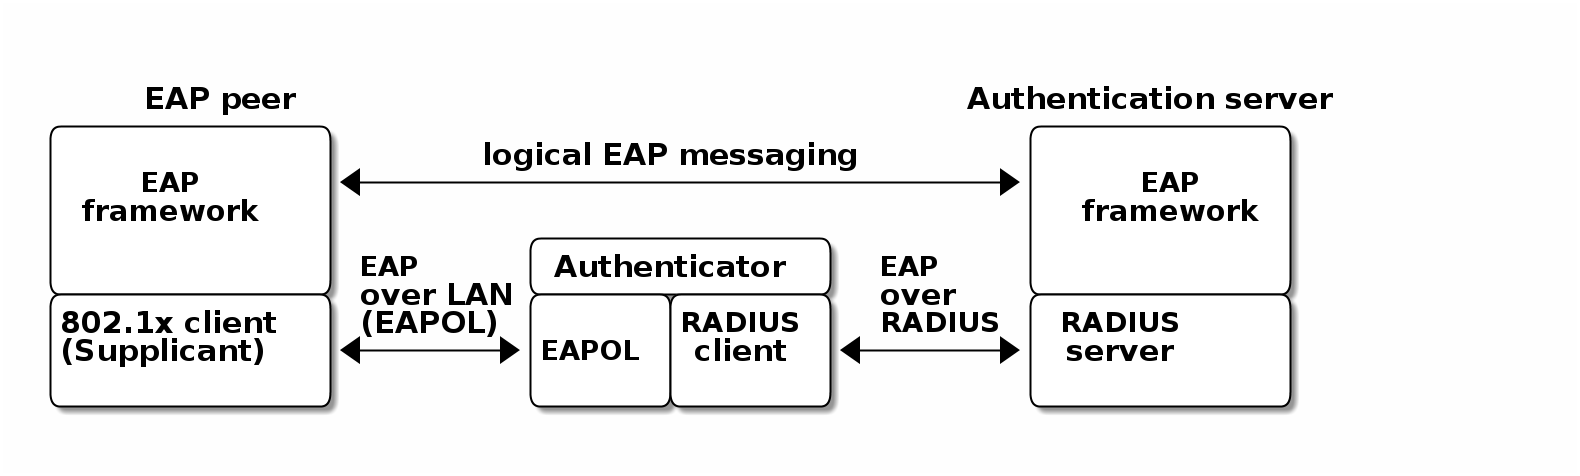
\includegraphics[width=.9\linewidth]{eap-layer.png}
\caption{\label{fig:eap-layers}EAP-logical layering}
\end{figure}






\section{SIM-based authentication}
\label{sec-2-5}

MNO and SIM trusts mutual each other.
There is still need for separate access credentials for Wi-Fi and
that was the reason of developing EAP-SIM and later derivatives
EAP-AKA and EAP-AKA'.
The goal was to combine in a secure way existing GSM keys for Wi-Fi
access. Existing general purpose EAP-methods in 2004 were not
compatible with GSM protocols for this purpose.\cite[p.93]{hav-doc}


SIM can be used via EAP-types EAP-SIM\cite{rfc4186},
EAP-AKA\cite{rfc4187} or EAP-AKA'(AKA-PRIME)\cite{rfc5448}.  
[ Write out this list]
\begin{description}
\item[{EAP-SIM}] EAP for GSM Subscriber Identity. RFC4186. GSM AuthN
protocol, network AuthN verified, if AP knows right
session key. Test cases on this work.
\end{description}

\begin{description}
\item[{EAP-AKA}] EAP for UMTS Authentication and Key Agreement
RFC4187. 3GPP-AKA protocol, mutual AuthN and network's
AuthN verified after receiving
EAP-request/AKA-Challenge. Values SQN and AMF from SIM
used for that. Incrementing SQN values eliminates replay
attacks.  This is not tested here.
\item[{EAP-AKA' (AKA-PRIME)}] RFC5448. Enhancement to AKA is to include
Service Set name (SSID) in the key derivation function. SHA-256
instead of SHA-1 digests.
\end{description}



  Using EAP-SIM means using secret key inside SIM card with A3/A8
algorithms to generate valid responses for challenges coming from MNO
and to derive session keys.  Algorithms used (A3/A8) and their
possible implementations (COMP128, COMP128v2, COMPv3) are not of
interest in this work besides the point that they are mobile operator
specific or known reference algorithms.
A3/A8 algorithm used in demo is called MILENAGE, which is a reference 
implementation and as such suitable for  operators who do not 
want to invent their own security algorithms.


EAP-SIM is similar to AuthN in GSM, but it adds mutual AuthN ie. also the network is authenticated.
Smartphone also sends in EAP-SIM a nonce, which is by definition a
value used only once, when network signs its response. 


In many parts, SIM variants in EAP are simpler, than other EAP
variants to mobile client.  Table\ref{table-peapsim} compares setup of Wi-Fi
in clients of one some existing organization compared to EAP-SIM. It
is noteworthy, that plain EAP-SIM will not support identity hiding and
that will be later be discussed further. If we add PEAP\cite{peap}
also to EAP-SIM, comparison will be more fair.
As can be seen from table, leaving certificates out from environment
makes client setup easier with price of revealing smartphone user's
identity.  



\begin{table}[htb]
\caption{\label{table-peapsim}Setup tasks in  WPA2-Enterprise with EAP-PEAP-MSCHAPv2 and EAP-SIM}
\centering
\begin{tabular}{llll}
 & EAP-PEAP & EAP-SIM & EAP-PEAP\\
Task: & with &  & with\\
(x)="needed", (N/A)= "not available" & MSCHAPv2 &  & EAP-SIM\\
\hline
choose CA & x &  & x\\
tell CA to clients & x &  & x\\
if CA not known, distribute it \emph{secure} & x &  & x\\
enable PEAP & x & N/A & x\\
set used EAP-method & x & x & x\\
set validating of RADIUS server & x &  & x\\
set encapsulation (WPA/802.1X) & x &  & \\
set outer identity & x &  & x\\
set inner creds & x &  & \\
hide identity &  & N/A & \\
\hline
\end{tabular}
\end{table}





Sequence diagram of full EAP-SIM authentication supplicant (here smartphone) and authenticator (in AP) is shown in figure\ref{fig:eap-sim-full}.
From the diagram we can see, that client's identity (IMSI) is
revealed in message 2 in plain-text. Later, client can use pseudonym to
hide its identity.

All EAP-SIM derivatives provide mutual authentication. Without NONCE
in message 4, that would not be possible. NONCE is by definition, once
used random string or number.
 Client challenges the network by
sending NONCE during start of the negotiation phase. It later checks in
message 7 whether RAND values from operator were digested with correct NONCE.

Yet some documents claim, that EAP-SIM does not provide mutual AuthN, so what
can be the case? Perhaps they mean, that mutual AuthN is not provided between
mobile and RADIUS servers. Another explanation is, that in AKA
and AKA' network is authenticated in very early phase with help of operator specific
symmetric keys, which are also inside SIM.





\begin{figure}[htb]
\centering
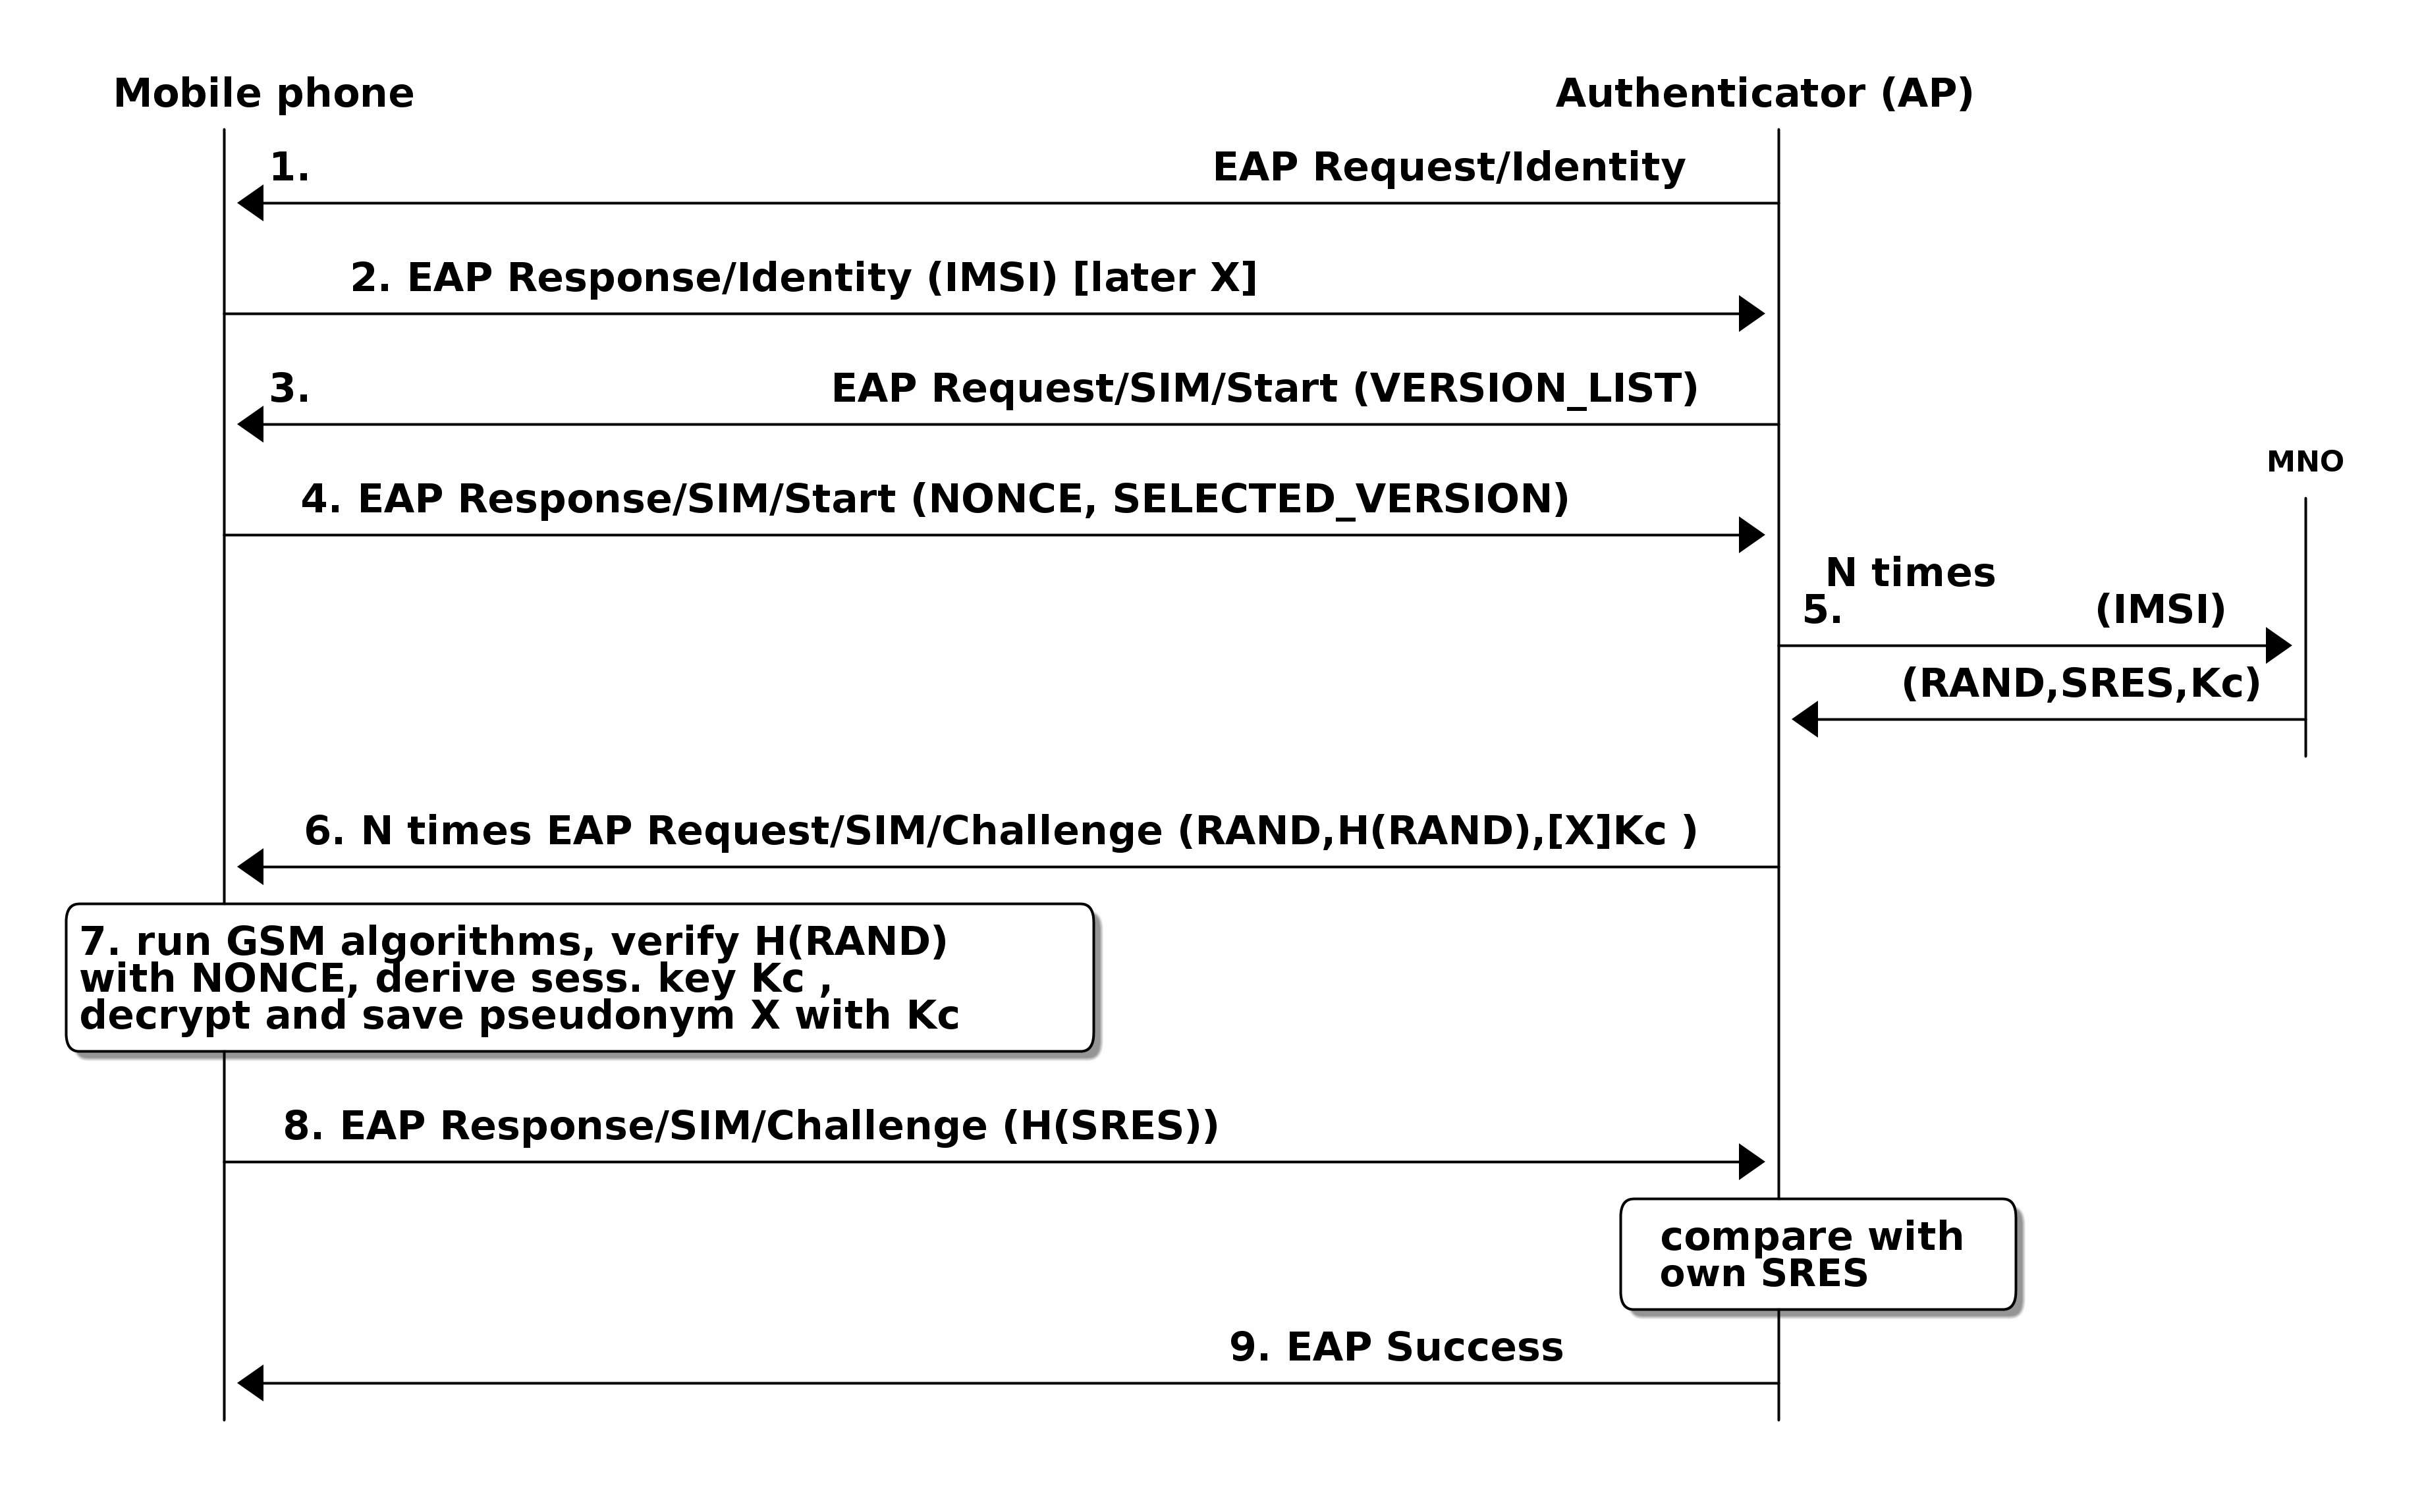
\includegraphics[width=.9\linewidth]{eap-sim-full.png}
\caption{\label{fig:eap-sim-full}EAP-SIM full authentication sequence diagram, based on RFC4186}
\end{figure}
\section{Trust}
\label{sec-2-6}

Trust is the base.
Secure communication has many layers. On its base lies trust. Without
trust there is little help with any added encryption or
secrecy. Setting trust is usually not an easy task, but only after
completing that phase it is meaningful to complete the other security
layers.
For example, secret keys enable encrypted communication, but the keys need to be
delivered through an trusted channel, and so it can be seen that trust
really is the first layer to be fixed. 



Even without trust, some form of secure key-exchange is is achievable
with Diffie-Hellman key-exchange\cite{diffie1976new}. Unfortunately, it is vulnerable
to Man-in-the-middle(MitM) attacks.  [MiTM discussed on IMSI-catching section]
With trust set between two devices, ie. if they can securely
authenticate each other, secret communication is possible. 
Secure network configuration and credential exchange is then possible.


\section{Security bootstrapping}
\label{sec-2-7}

[NOT YET trust anchor methods HERE!!! ]

Bootstrapping protocols are used to bring first trust anchor in an
environment and use that device to attach other devices to same trust
circle. Despite its name, bootstrapping usually needs some information
from outside. 


 [Evaluating and comparing bootstrapping methods and authentication.
Evaluation missing, so comparing difficult too.]

[Description of General Bootstrapping architecture (GBA) vs. yet
another custom architecture. Maybe parts of architecture
such as using SIM-auth (EAP-SIM) or CallerID, how they differ. 
What is needed? How GBA could be used here?
Any other authentication methods such as CallerID
as a primary identification (bootstrap) and later as identification?]*

[SIM card's anatomy: it has private key, MNO
also has the same key in its database and that is used to derive
other keys based on input received.]


As shown earlier, 
the mobile phone and MNO trust each other hence mutual authentication
between them  is possible.
  How this can be used to include other components in the homenet? As AuthN-AuthZ at home
proceeds through authenticator, maybe authenticator can deliver this information
further and use it as a derivation function to extend trust.

EAP-SIM derivatives provide strong AuthN meaning here two-factor
authentication. Software certificates, while stronger than passwords,
do not possess properties \emph{non-copiable} or \emph{unique}, so they can only
be considered as a strong password.  
If we nonetheless were using software certificates with method such as
EAP-TLS, then the certificates (for CA and client) and the private key
should still be provisioned first, which would defeat what we wanted
to achieve.
\chapter{Managing Home Networks}
\label{sec-3}
[ keep this security oriented, Forget sections \& subsections style.]

\section{Home network architecture and IETF}
\label{sec-3-1}


Home network is computer network located at person's home. It consists
of devices and their interconnect, either wired or wireless.  This
thesis denotes home network as homenet, although the name 'homenet'
is reserved to Internet Engineering Task Force Working Group (IETF WG) homenet.
IETF is responsible for the most Internet technology standards.
Current drive in homenet management is towards IPv6 environment
 as it allows future  addressing and routing needs. As old technology
cannot be forgotten, homenets will be heterogenous having both
old and new technology and their interoperability is important in
planning future homenets. Segmenting home in multiple subnets will belong
to homenets and will include areas for home members, guests,
and management.



Securing homenet and its router's configuration is done by limiting
traffic with static or dynamic access control lists (ACL) in
routers. ACLs in turn are secured from change by AAA. Authorized
agents can make changes, either direct in the device or through some
management protocol such as SNMP or NETCONF[source].  SNMP has been in
use for over 30 years and well supported in routers. Only there are
multiple version for this protocol. While earlier versions (v1, v2)
did not provide any encryption of messages version 3 knows for example
about public keys and is secure enough when used correctly.


Management of devices on border of homenet and operator have 
been done already earlier. For example TR-069 standard
exists\cite{iptvtr069} for CPEs such as ADSL broadband routers or
set-top boxen. TR-069 has been used to implement self-configuration
archi\-tecture in
homenets\cite{tr069rachidi2011}.
On these days research is done with Light-weight Machine to Machine
(LWM2M) processes. 


RFC7368 about IPv6 Home Networking Architecture Principles from
Arkko\cite{rfc7368} defines the borders of the homenet and states that
internal borders in homenet should possible be automatically
discovered but continues by saying that limiting borders to specific
interface type makes it difficult to connect different realms locally.
The same document continues stating
that while homenet should self-configure and self-organize itself as
far as possible, self-configuring unintended devices should be
avoided and let homenet user decide whether device becomes trust.
So, these statements reveal us that homenet environment still needs
external configuration even with proposed automation aids.





Authentication (may) need some bootstrapping of trust for start.
Homenet WG proposes use of PKI in the home.  To use PKI, bootstrapping
protocols are first needed for trust anchoring.  Behringer's
draft\cite{draft-behringer-bootstrap} proposes, that first one device
is chosen for the trust anchor and trust is built upon that
anchor. This anchor device then becomes homenet's Certificate
Authority service. In the end, rest of the homenet will be imported
into homenet through CA, which signs their certificate requests.

Key creation, key exchange and their usage is explained in similar
draft from Pritikin\cite{draft-pritikin-bootstrap}. There is also discussion about using
manufacturer provided device certificates as trust anchor.  If EAP-SIM
was applied in such environment, it would be used only once, namely in
the bootstrapping phase to setup the CA trust anchor.  The public key
cryptography is processor intensive and its asymmetric keys are
usually used just in the beginning of communication. There they can be
used to securely negotiate symmetric keys which allow faster
cryptography processing. [source?]


This model could also be expanded to full ticket enabled
Kerberos-style network, where time-limited tickets (tokens) exist for
both authentication and authorization for different services. Trusted
Third Party authentication center would be setup with help of MNO.
One service would then authenticate an entity, here smartphone and
give it time-limited ticket as prove that the entity has been authenticated.
When the entity wants to connect to service, it asks from central 
server again ticket but this time for service by presenting
authentication ticket. In return it receives service ticket and that
it can present to wanted service.






Homenet configuration itself is excluded from this work.
That includes configuring power level setting of devices to save electricity
based on usage profile. For example at nights or when there are nobody
home, some devices don't need to be working at their maximum
capacity. Instead, we study interface of AAs.  Main points here
are existing infrastructure(phones, Internet access, Wi-Fi
access points), strong authentication (two-factor) and existing
authentication methods (EAP-\{SIM,AKA,AKA'\})
\section{Centralization trends in management}
\label{sec-3-2}

Traditionally, management of network devices has been done
individually using each devices console or web-access.  As number of
devices has increased, it would have been reasonable to rationalize
the process by central management device, not least to prevent human
errors for repetitive tasks.  Yet, at home networks devices often are
too heterogeneous, bought at different times from different vendors
and so incompatible with each other to fully benefit from
centralization.

To help moving the management to the more centralized model,
smartphone is set here as a central and managing local controller.


Users already have one phone, which can be considered as
'smart' and most smartphones have Wi-Fi capabilities and suitable for 
Local Controller between cloud and homenet.
When we choose smartphone to be the management point, the other benefits are
numerous:  management software can be delivered and
updated from cloud to diverse smartphone types, and existing user
base is enormous.
Operator located user databases (HLR-AuC) still have orders of
magnitude more users available than any organization. 




\chapter{Design of home network trust anchor}
\label{sec-4}




[chapters contents here]

Key distribution problem is solved at SIM-card distribution phase.
SIM card authentication is strong: there is physical SIM and secret PIN for it.
Smartphone then belongs to same category as (intelligent) USB-dongle,
RSA-ID or Secure-ID hardware devices.  They are part of "what you own".
Trust exists to mobile operator, and that is later shown as an
important factor. 



Disadvantages with SIM is dependency on mobile operator and internet
connection, although disconnectivity issues are later addressed partly.
Using smartphone may cost money, either to client or to service
provider, although costs could be lower than using SMS, because 
IP network is used instead of mobile
phone network.


The smartphone connects
 with Wi-Fi link to access point (AP) in homenet.
 AP functions there as an authenticator.
Trusted connection is needed between existing network and Local
Controller ie. homenet and local controller need to trust each other.
Smartphone will approve changes for homenet and is part of bootstrapping
new infrastructure.

\section{Alternative methods for introducing trust anchor into the homenet}
\label{sec-4-1}

Before fully explaining our chosen method, we introduce some
alternative approaches for trust anchor. Trust anchor is part of
bootstrapping. Trust information, may it then be a secret or some
evidence, can be delivered to trust device via physical
transport. Traditional way to do that is with password inside sealed
envelope or one-time password list what online banks today use. Secret
can also be sent as an SMS.

Trust can be requested with help of trust anchor's unique
 properties. Some new devices have vendor certificates inside them which
brings public key infrastructure as possible alternative. Device
presents itself with a certificate, which has been issued by a trusted
vendor.  Keys are then in device's trusted hardware store.
Vendor-trust is needed for checking issued certificates. Root CAs, 
trust anchors also, can be read from device's read-only store. 
CPE could use vendor certificate for AuthN of earlier unknown device.
If keys are stored in SIM as here, external operator support is needed. 


Other techniques than EAP-SIM to use SIM's unique properties
are for example 
Bluetooth SIM Access Profile(Bluetooth  SAP), 
direct connection through PC/SC (Personal\-Computer/Smart\- Card),
CallerID service from phone network, and
Mobile signature service such as "Mobiilivarmenne" in Finland.



Bluetooth SIM and PC/SC would need patching of smartphone's software
to work.  On the other hand, the smartphone would any way need to
download controlling application
in the beginning for advanced use, so these techniques could be
studied further in another work.

Caller ID as an authentication method uses GSM-network's controlling
channels. When a phone makes a call, the receiving end gets 
to know callers phone number (ie. IMSI) before it answers the call.
That information is called "Caller ID" and it has been is use
successfully for some door locking implementations. 
It does not cost anything for caller or responder,
because after receiving the CallerID  information, responder can hang
up upcoming call and no call expenses are created.
 It can also be made safe at least in Finland
by limiting which tele operators are allowed to connect.
















European Telecommunications Standards Institute (ETSI) defines
standard for mobile signature services (MSS) in ETSI TS 102 204.
MNO's in Finland have implemented this as a "Mobiilivarmenne"
service. 
For example, Sonera's brand for  it is "Sonera ID" while Elisa calls it
"Elisa Mobiilivarmenne".

When AuthN and AuthZ comes from outside, one possibility is to use
federated Mobile AuthN Service, which then is connected to MSSP(Mobile
Signature Service Provider) with ETSI-204. Benefits for ETSI-204
federation is that no single home device must implement it at home,
but also MNO sees service as just one client.  Without federation,
mobile AuthN services would need to be multiplied with number of
clients.


[Project Moonshot for federated ssh-access? NOT HERE]
\begin{quote}
Moonshot is a technology, based on the IETF ABFAB open standards, that aims to enable federated access to virtually any application or service.
\end{quote}
source:\url{https://wiki.moonshot.ja.net/display/HOME/Home}
[Moonshot, if worked and used together wit MSSP, may offer SIM-based
ssh-access to Authenticator.] Possible modifications needed on SSH
server and client.

At this point question might rise, why these external service
providers are needed. Is it not easier and simpler to just send 
an SMS with password code to mobile, when access confirmation is needed?
Mobile SIM provides two-way AuthN part as discussed earlier.
Without need for strong AuthN, that model would indeed be 
simpler, but using SIM also solves initial key distribution problem.
Additionally, mutual AuthN problem would still need to be solved:
Who sent that password?



All this time it is assumed, that hardware does not lie. In case
the hardware has been tampered, we could not trust it and its claims.
For example, there have been attacks against SIM to reveal its private
key after SIM have been copied.  To verify, that a device has not been
tampered, method called attestation is used.

A device which has attestation capability such as 
hardware certificates or Trusted Platform Module (TPM) technology
can be function as a trust anchor.
Such a device could be sent direct to customer with pre-configured
secrets and methods to take a place as a trust anchor. 
That leads us again to key distribution problem.






Phone brings trust to homenet by completing full EAP-SIM AuthN through
local Authenticator. SIM's identity is verified by HLR AuC at phone
operator's end. Verification leaves a trail on local authenticator and
opens trust channel for limited period of time for changes from the phone.
[This was the most important paragraph of whole work. Thanks for
reading it.]





In this implementation, no extra application is needed in smartphone
for primitive trust, but later for more serious use some application is needed.
Requirement for homenet can be as small as having WPA Enterprise capable
Access point. Almost any AP will  do, but as an exception, cable modem Bewan, which 
has been distributed to many homes from the operator, was found to have only WPA2-PSK mode.
Additionally, managing user's SIM-card has to be registered as an admin user in homenet 
configuration ie. its IMSI must have admin rights.


 For added functionality, for example for
logging admins out, OpenWRT based hardware can be used, although those functions have
not yet been implemented. 
[See "disconnect" section below on chapter xxx]

[picture?]

\section{Flow of design (already above)}
\label{sec-4-2}

Wanted: 
\begin{itemize}
\item separate MGMT net exists
\item SIM authentication to MGMT net is proven
\item changes are authorized if they come from MGMT net
\item log-out from MGMT net
\end{itemize}
(- spare connection, if internet link down)
(- fast-reauth, without MNO

Implications are, that when someone has access to MGMT channel,
everything is permitted. No security limiting as default 

[Basically 2. and 3. is like traditional corporate network with firewall.]

a. AuthN is proven

b. AuthZ decision has challenges

c. Change approving has three cases:
\begin{enumerate}
\item Changes are allowed, when port is open
\item Confirmation message from MGMT-net authorizes changes.
Message must belong to configuration and can be example a digested signature.
\item FULL: changes may come only from MGMT net.
\end{enumerate}


Use-case for adding admin user:

Let's first suppose, for case of simplicity, that the homenet has been
already configured(bootstrapped) and it is functioning properly.  The
home configuration model has been copied[inserted, etc] to the cloud.
When changes are made to the cloud model through authorized cloud
administrator users (operators), those changes are later also committed
in to the production in homenet. There is no magic here, plain
configuration change, just this time externally initiated.

Now, let's think what happens, when the cloud operator (or owner of
homenet) tries to modify attributes, which give access to new actors,
such as new operators, who would want to have access to separate
segments of homenet.  First we need to have that segment separation
change approved and after that we want to allow the newcomer account
to have access to that segment and only to that. For the first part,
which is normal operation, approving would perhaps yet not be
necessary, but for the second part we need some checking unless our
trust to cloud operator is ultimate.  [FOR approval needs, discuss
this with the team.]



Changes could be marked some way, so that they need approving.
When CPE of homenet is about to input configuration
changes which would change balance of authors or roles,
it will first need to ask for permission. 
It does it by asking from trusted point, here mobile SIM. 

[How is this PULL asking triggered? In reality it is not asked, but
changes are accepted from admin roles. How admin role is checked?]

CPE wants to verify if the changes authorized. They are, if currently
smartphone user is logged in management network (ie. management is allowed).
Additionally, there could be a  specific change-approval message,
which must be sent through  management network, maybe
including digest of change message as a verification and.

Because smartphone is not actively listening the CPE, how it could
input that request? 
There are three planned ways to distribute changes.

\begin{enumerate}
\item Changes are delivered normally from cloud to CPE (CPEs) without
interaction  from the smartphone. Such changes would not need
AA at all.

\item Changes are delivered from cloud to CPE functioning as a central
management station without interaction from the smartphone. 
Digest of what is going to happen would be sent to smartphone from
BaaS. Smartphone would authenticate (if not already ) in to
management network and send through it the digest token it received from cloud 
as an approval message to central management station
inside homenet, which then forwards configuration changes to other devices.

\item Changes are delivered from cloud to smartphone, which after
authenticating into management net, forwards them through management
net to each and all devices.
\end{enumerate}


The smartphone may receive authentication token with (not
authorization, but )message explaining what is going to happen in the change.
As the CPE and the authenticator may be separate devices, approving
happens by sending the token from the smartphone to the CPE via the
management network where authenticator gives access.

It must be noted, that the smartphone can already have an association
to a non-management network with Wi-Fi. If that is the case, it first
must disconnect from there and then connect (ie. AA) to correct management
network. That implies disconnection from other services, because 
smartphone currently has only one Wi-Fi radio available. 
It is not tested, whether 3G-data link could be active still at the
same time.



\section{Chosen Design and why (Rationale)}
\label{sec-4-3}

Network can be divided into separate segments. 
First, there is normal access network which provides
connectivity. Second, there is network through which devices are
managed, so each device need to have at least two connections: one for
access and one for management. It is not defined, if those connections
are physical or virtual (VLAN's etc). 
Analogy to real world would be public access corridors and doors for
customers separate from privileged doors for service personnel.

Access to segments is checked in routers with access control lists
(ACL), where decision is made based on current configuration or user's
role.  Once user has been authorized into management network, access
stays open for him, at least for (predefined) limited time.

So, instead of checking user's credentials each time data is received
this model only checks, from where data is received. 
Data received from management network is granted for changes.
It is arguable a lighter method than always
fully AuthN and AuthZ but may suffice here, at first.

Naturally one will first challenge the solution, if
management network is thought to be in secured zone.
but sure devices have additional protection for logging in them. 


Example of complex solution would be a traditional firewall and packet
inspection in interconnects. Even more complex would be that traffic
always travels through Access Control Engine such as Google's
BeyondCorp\cite{2014-beyondcorp}, where all
traffic is suspected as being external, even when it originates from inside networks.

In production, some changes in cloud are propagated to homenet via
management network without need for extra authentication phase.  [This
was mentioned somewhere, move here] Those changes or alternatively
changes that do need authorization should be enumerated, which ever
would be smaller set. In our model, [only] initial bootstrap needs the
authentication with smartphone as does changes in roles and some
dangerous combination of commands.

It is desirable, that no local change in homenet be done because of
synchronization issues [-> see later, if synch. section written],
but that will rise question for further studies if synchronizing algorithms such
as Trickle are used in homenet.




When homenet needs secure binding to the mobile controller, earlier
mentioned trust is the first one needed.  The trust is achieved by
checking whether the mobile controller can access home management
network only with its trusted SIM-card, which provides AuthN. AuthZ in
turn is compared to existing roles in authenticator.


[This has been explained]

Technically we use in Wi-Fi connection IEEE 802.11i, which includes
802.1X as port based access protocol.  802.1X defines there
authentication, authorization, and cryptography key agreement
\url{http://www.ieee802.org/1/pages/802.1x-2010.html}. It uses
Extensible Authentication Protocol (EAP) which selects specific
authentication mechanism\cite[p.3]{rfc5247}, after Authenticator
requests smartphone to identify itself as in figure xxx is shown
Messages are carried over 802.1X or RADIUS depending on transport
medium as of figure [picture drawn for layers earlier].


When AP forwards authentication request to next RADIUS server, it can
ask or receive, beside AuthN and AuthZ, other service parameters, such
as provisioning. That would allow the smartphone to connect to
specific management network access either via CLI or SNMP or similar
\cite[p.4]{rfc5608}.  RADIUS can bring extra attributes in its
ACCESS-ACCEPT message.  Specific VLAN attributes can be delivered via
Vendor Specified Attributes (VSA) or similar 'getting into VLAN'
attribute, if standard RADIUS messages do not suffice.  VSAs allow for
vendor to use extra 255 attributes as they wish, but also currently
there exists RADIUS extensions for directing user into VLAN [cite
rfcXXX].  That way authentication server (3rd party) can divert and
segment areas of home network.  In our case, admin users are put in to
the management network.
  Yet usually RADIUS ACCESS-ACCEPT message which means AuthN and
AuthZ were successful already allows user to access wanted network. As
for other provisioning parameters, not all end devices support them.

[ VLAN membership could be given during AuthZ to mark belonging to the
MGMT-VLAN.]  





In Behringers work-in-progress  bootstrapping\cite{draft-behringer-bootstrap},
AuthZ happens likewise first at cloud providers
end, but after checking devices Vendor certificates cloud provider
gives device a ticket of authorization like in Needham-Schröder or
Kerberos implementations. Device presents that ticket to CPE which
finally can decide, whether it allows change. 
Here, instead the authentication server can be external RADIUS server,
but usually the final decision point lies at authenticator in CPE.
[?]


\section{Access methods to Wi-Fi with only one SSID}
\label{sec-4-4}
Today, homenets usually consists of only one Service Set ID (SSID)
Wi-Fi network though it is possible to define multiple SSIDs in
access point. Having multiple SSIDs enable us to dedicate one of them
to management network. 
To enable EAP-SIM method, it is necessary to use WPA-Enterprise mode
an as such, to use RADIUS server.

It was not found, how authenticator could use the same network with
both WPA-PSK (or open access) and WPA-Enterprise, so
this separation is only technical.


If Wi-Fi were limited to only have one SSID then we would need another way
to separate access requests to management net.  Access to Wi-Fi can be
separated by multiple realms (different username domains), different
authentication methods, or it can be based on user role.
\begin{itemize}
\item Normal access, no RADIUS or just plain backend.
\item WPA2 Access, shared secret, no RADIUS
\item PEAP access with whatever EAP outer-inner encapsulation
\end{itemize}
encapsulation was explained on xxx





Wi-Fi Alliance has certification program (Passpoint) for Hotspot2.0 compatible
devices.  Hotspot 2.0 enables selection of network based on ownership,
services and performance characteristics \emph{before} Wi-Fi client has
been associated to Hotspot 2.0 AP. The technology is built on
IEEE 802.11u specification.


Ownership, service and performance characteristics?
One could guess, that they are
\begin{description}
\item[{ownership}] costs, money
\item[{services}] sound, video, IP, printing, etc.
\item[{performance}] speed and latency
\end{description}

It is well known, that usability of Kiosk-mode Wi-Fi
 networks is burden, because user needs to go through 
web portal logins with username-password authentication 
procedure and those are different for every network.

In 
\url{http://www.ericsson.com/res/thecompany/docs/publications/ericsson_review/2012/er-seamless-wi-fi-roaming.pdf}
goals are to smooth roaming between Wi-Fi and 3GPP/LTE networks
an bring operator-grade to Wi-Fi by putting control in operators side. More
than offloading traffic, plans are to bring other services also to Wi-Fi.

TO DO: check 802.11u features and what they add to 802.11-2007
\begin{itemize}
\item interworking with ext networks
\item hs2.0 is extended 802.11u
\item next generation Hotspot
\item advertises external networks \emph{before} association. no need to
select Service Set ID (SSID)
\item access network type, roaming consortium support and venue information
\item some QoS mapping
\item emergency services (not in HS2.0)
\end{itemize}


\section{Scenarios for authorization (AuthZ)}
\label{sec-4-5}

[Place of Authorization decision  ]

AuthZ decision usually happens at home.
If the decision is made on remote AuthN server, 3rd party, 
then that server needs to have access to cloud service's AuthZ data. 
Further it seems inevitable, that just like the homenet model
having AuthZ data of eligible IMSI accounts  is in the cloud, 
then also delegating AuthZ to cloud simplifies homenets
functions. Instead of putting logic on CPE for AuthZ, CPE
could just trust the 3rd party service's AuthZ message, which is 
RADIUS message of either \emph{ACCESS-ACCEPT} or \emph{ACCESS-REJECT}.


Here are presented 5 scenarios for possible locations of AuthN and 
AuthZ points. Authenticator is the entity which gives the final decision 
about access. In most cases it is the located in the
local AP, but it  can also be external, like in scenario V in 
table \ref{table-scenarios}, where locations for Authenticator (AA),
AuthN, and AuthZ are marked as (I) for internal or (E) for external.

\begin{table}[htb]
\caption{\label{table-scenarios}Location of AA, AuthN and AuthZ in scenarios I-V}
\centering
\begin{tabular}{llll}
scene.no: & AA & AuthN & AuthZ\\
\hline
I & I & E & E\\
II & I & E & I\\
III & E & E & E\\
IV & I & E & E\footnotemark\\
V & - & - & -\\
\end{tabular}
\end{table}\footnotetext[1]{BaaS provides}

\label{scenario-i}
The first AA-scenario is presented here thoroughly as an example.
The goal is to make trusted configuration change. 
The steps are numbered in figure\ref{fig:scenario-I}.
Configuration change is allowed, if CPE gets ACCEPT from MNO.  MNO gets
information of allowed users from Cloud (BaaS [def.])


\begin{figure}[htb]
\centering
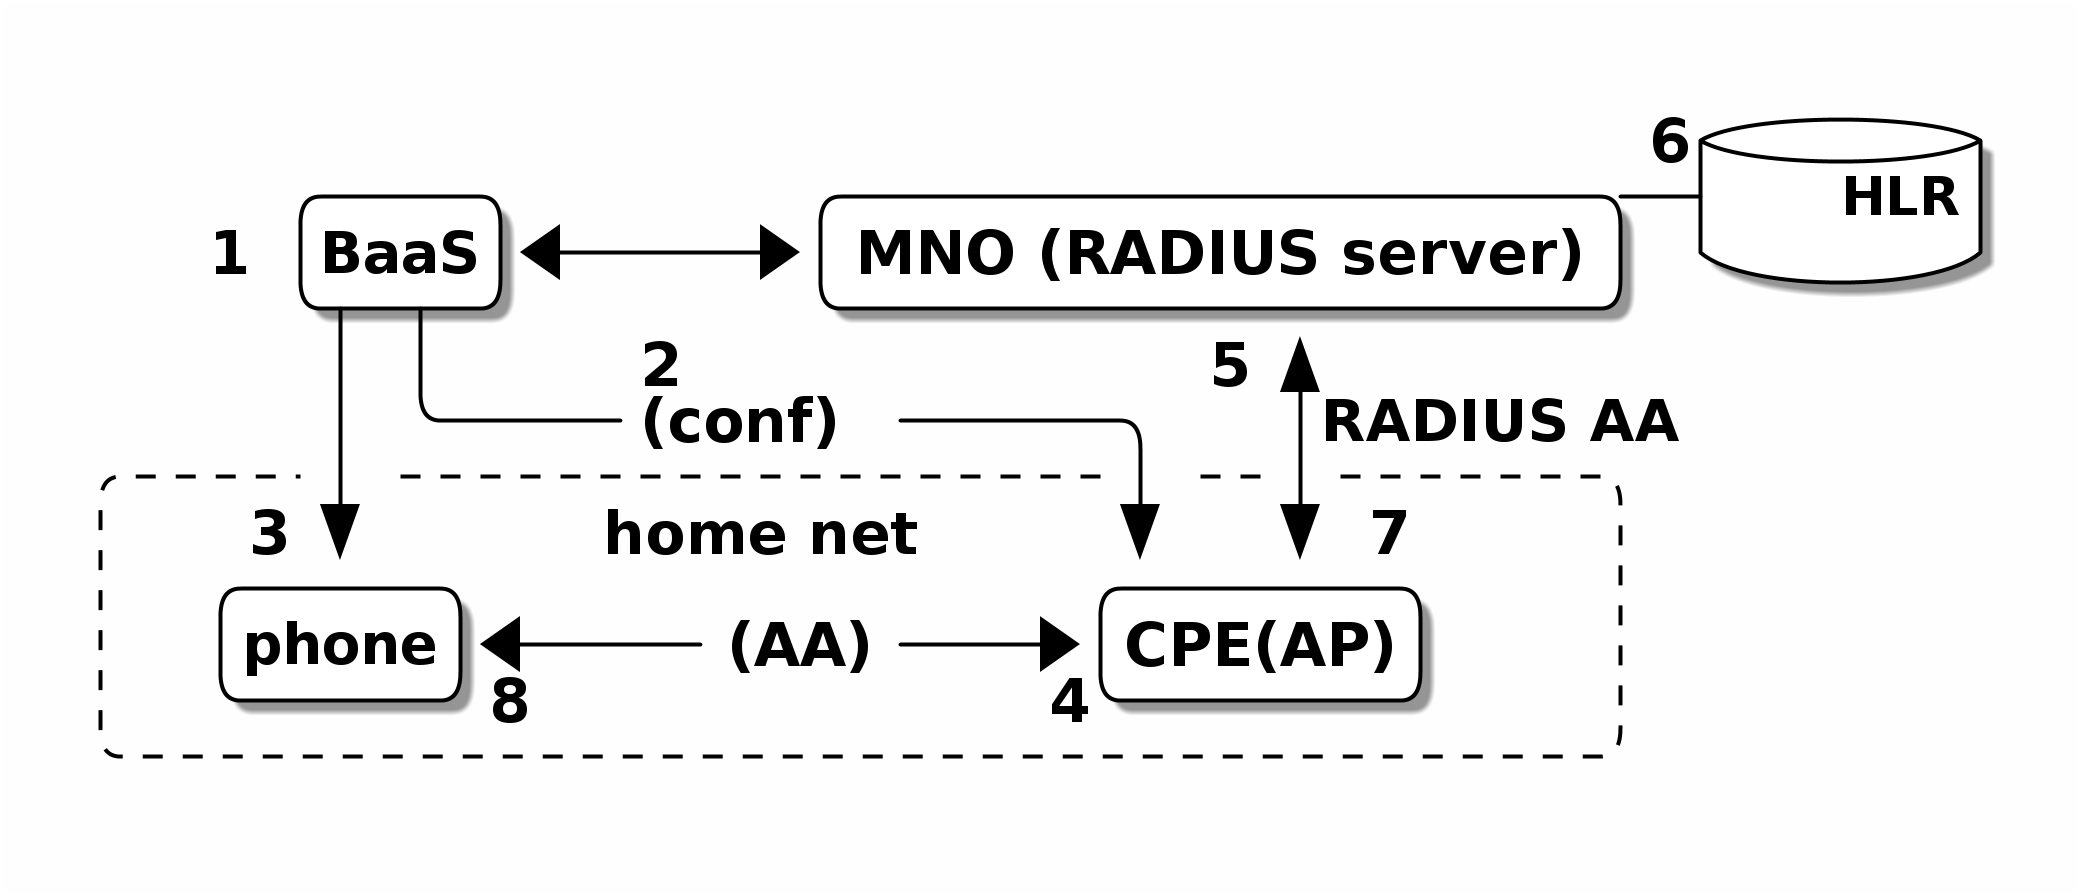
\includegraphics[width=.9\linewidth]{scenI.png}
\caption{\label{fig:scenario-I}Scenario I with 3 separate domains: BaaS, MNO and homenet}
\end{figure}


\begin{enumerate}
\item The model has been changed in the BaaS.
\item BaaS send changes to CPE.
\item If changes are privileged, they need to be approved by phone user.
Changes are sent also to the phone and phone user must authenticate
itself to the management network.
\item Phone user starts authentication process to management
network using EAP-SIM and reveals its IMSI.
\item CPE  (AP) forwards authentication to MNO's RADIUS server with
RADIUS protocol
\item MNO have RADIUS server running and it authenticates IMSI user with
  its HLR-AuC.
MNO also asks from BaaS, whether IMSI user has admin-role (AuthZ). [how long does it take to ask?]
MNO returns in RADIUS message either \emph{ACCESS-ACCEPT}, if user is both known AND has admin role 
  or \emph{ACCESS-REJECT}, otherwise
\item CPE receives this ACCEPT or REJECT. If there were other RADIUSes
between CPE and MNO, they would have acted
as proxy RADIUS servers.
\item IF ACCEPTed, then mobile is both authenticated and authorized and
can send configuration change message to CPE, which recognizes it
coming from authentication network.

While changes has been already sent to CPE direct and only let it
wait for approval, then when CPE receives ACCESS-ACCEPT, it could
already proceed on propagating those
changes.  Otherwise, after certain timeout, CPE must stop waiting
for phone's approval and drop changes. [this was the question
somewhere, "triggering"]
\end{enumerate}

This simplification has pitfalls. If mobile stays in management
network continuously, how are upcoming changes separated? Mobile should
either be dropped out from management network right away after changes or
after predefined timeout period.  If on the other hand, mobile must
send changes itself, then it would be possible that access in the
management network has short period of time, when phone 
holds that status or acceptance token. For example for 10 minutes connection
would be open for changes. Then changes would not go directly to CPE
but instead to , but they would include some token to phone, which is
needed for approval message.


\label{scenario-ii}

In second scenario (Figure\ref{fig:scenario-II}), AuthN is asked from MNO but
AuthZ is checked from local database. Local data comes from data model
ie. from configuration data and will be saved in CPE, or some other
place within homenet.


\begin{figure}[htb]
\centering
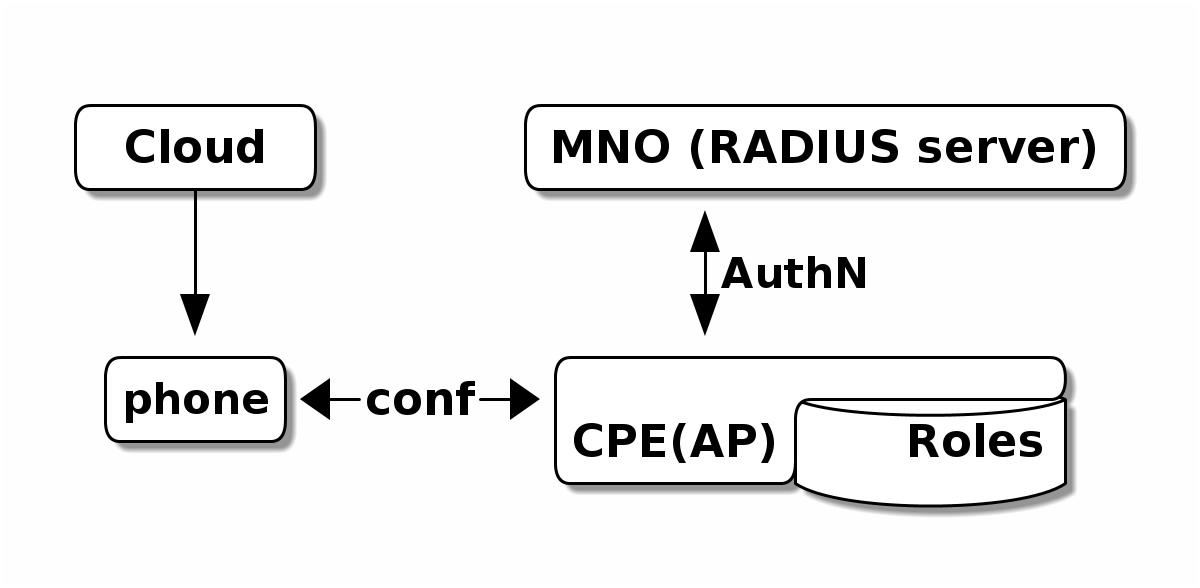
\includegraphics[width=.9\linewidth]{scenII.png}
\caption{\label{fig:scenario-II}Scenario II with AuthZ in homenet}
\end{figure}


\label{scenario-iii}

Similar to first scenario is scenario III (figure\ref{fig:scenario-III}), 
but this time there is SP between CPE and MNO, so AA is fully outsourced:
local AP communicates with RADIUS-protocol to the external
authentication server. That in turn gets AuthN from MNO via its
hlr-auc-gateway and AuthZ from BaaS.
Locally there is a cache for roles in case of network disconnectivity.

Here benefit is, that 3rd party authentication server may have direct
contracts to many MNOs, so user does not need to find and choose
them. As a bonus,  MNOs already delegate requests to right operator, if
they happen to get AuthN request which does not belong to them.
This is similar to federated service.

\begin{figure}[htb]
\centering
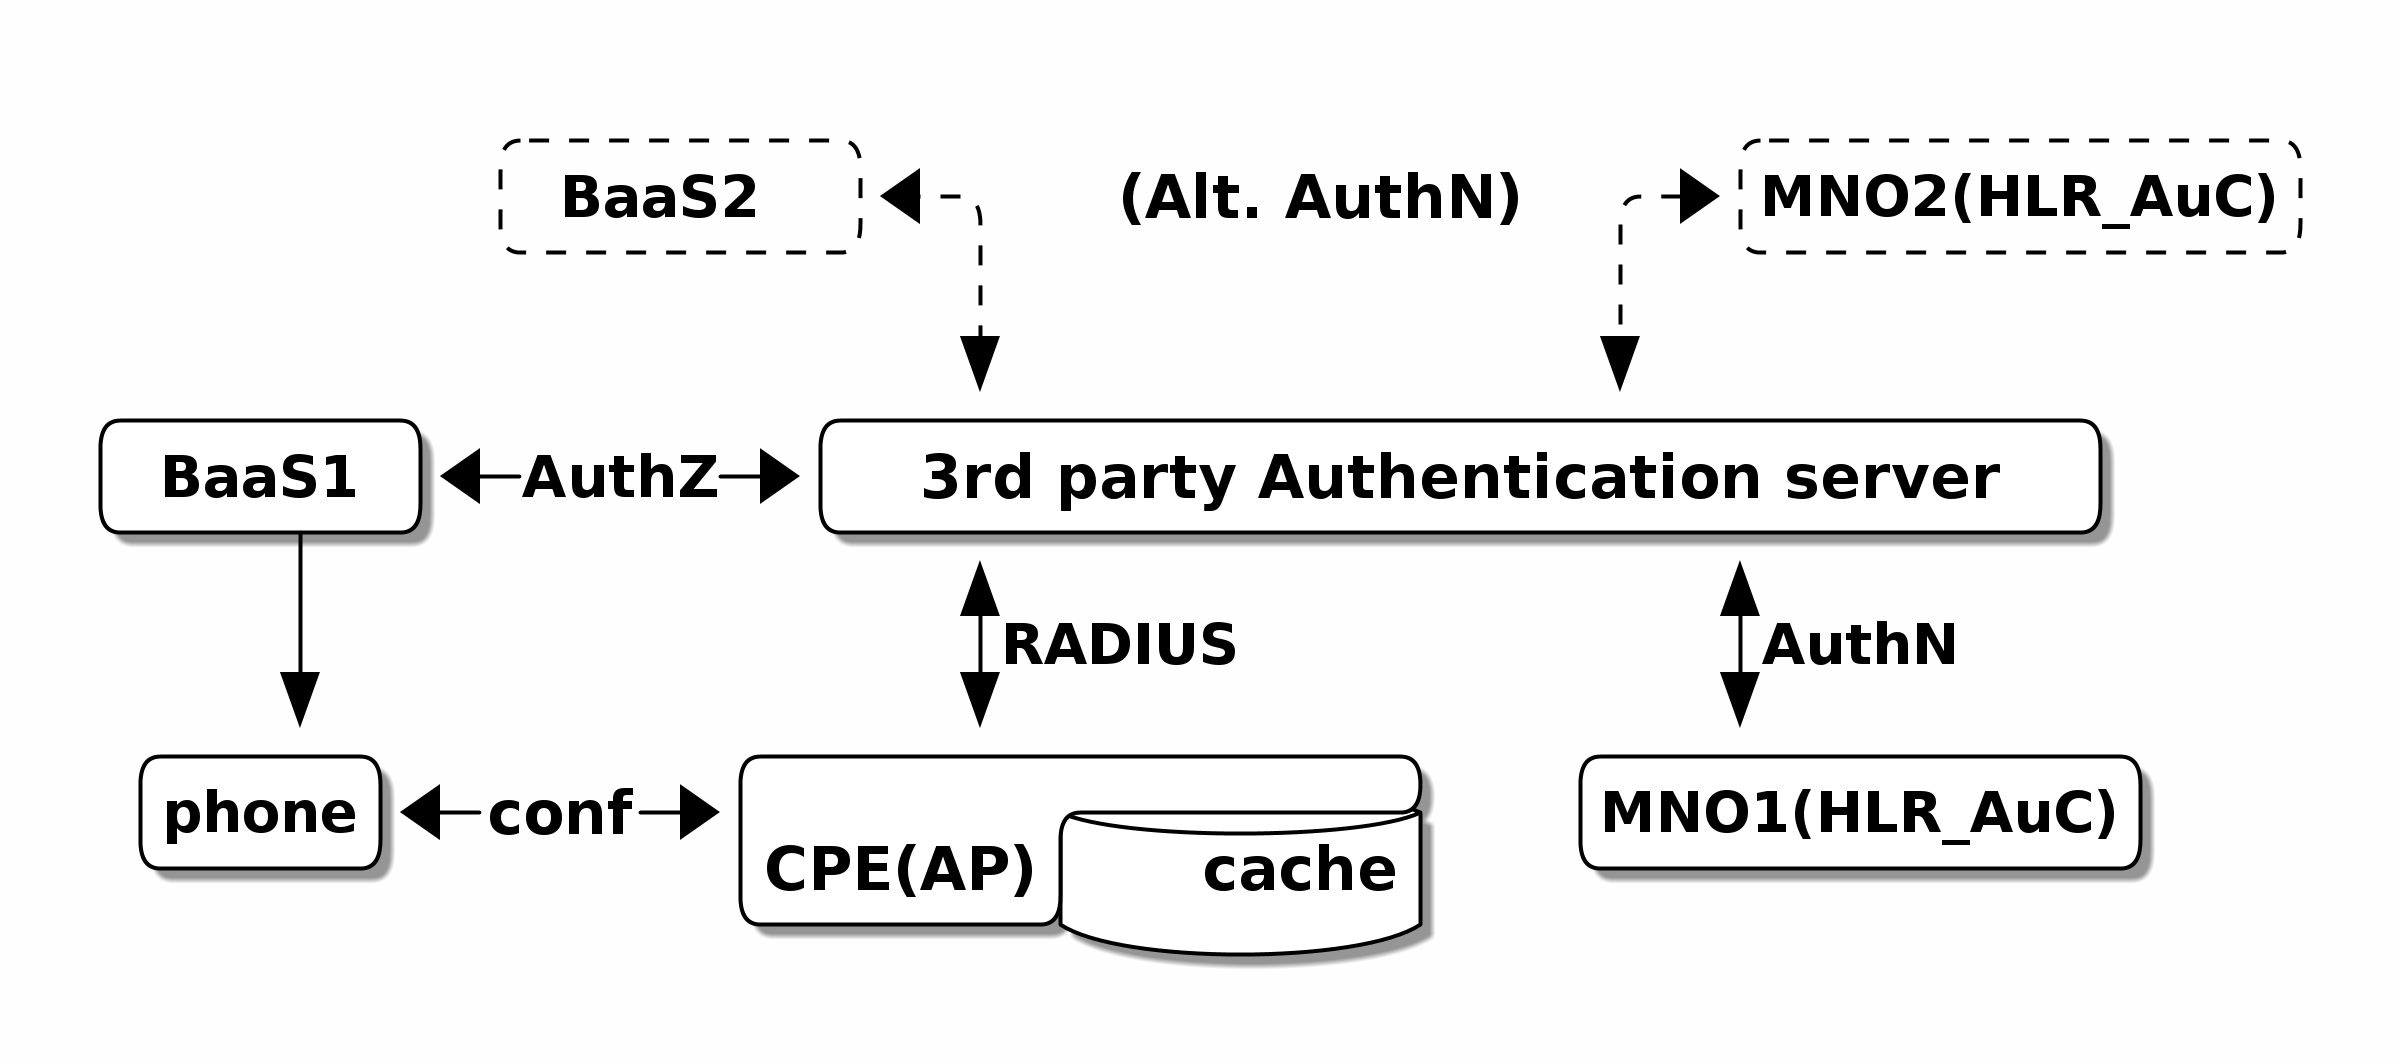
\includegraphics[width=.9\linewidth]{scenIII.png}
\caption{\label{fig:scenario-III}Scenario III with outsourced AA}
\end{figure}

Allowed users are verified from BaaS's registries and specific IMSI is
authenticated from MNO.  It may need some preparation, if SIM
identities are temporary ie. TMSI is used.  Still, IMSI is carried out at first message
of full authentication. Later, the server would need to have mapping
between IMSI and TMSI, but because only full-authentication is used,
there should be no problem.
[ That is, it is possible, that not every change needs
authentication.]
[ move that sentence elsewhere]


\label{scenario-iv} 


Scenario IV (figure\ref{fig:scenario-IV} is almost like scenario II, but
AuthZ is always checked from BaaS. If there are no connection to
cloud, fall-back is to work as II. So also this scenario needs local
store for admin IMSIs.

\begin{figure}[htb]
\centering
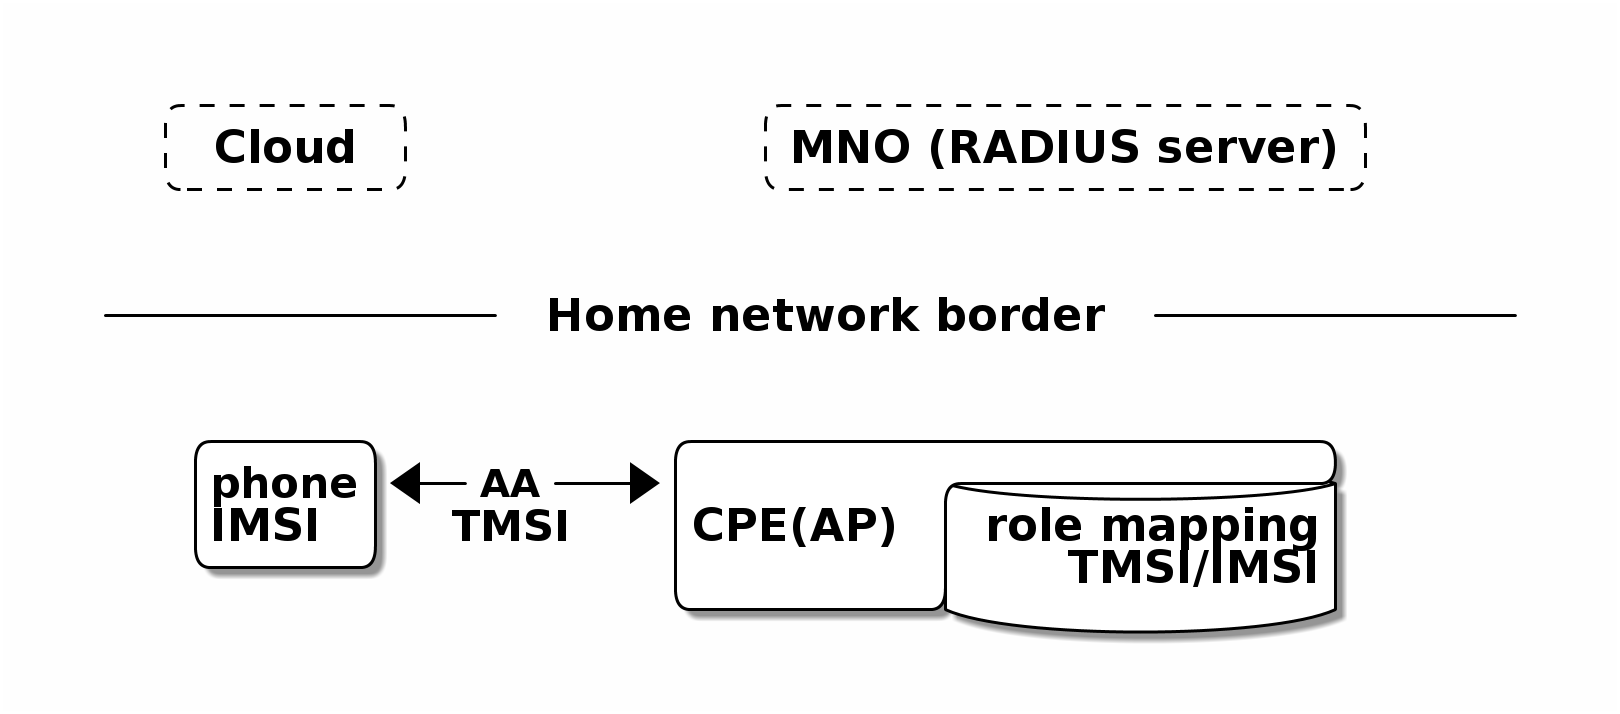
\includegraphics[width=.9\linewidth]{scenIV.png}
\caption{\label{fig:scenario-IV}Scenario IV, AuthZ from BaaS, AuthN from homenet}
\end{figure}

In last scenario (no figure), nothing has yet been configured. The bootstrapping
is not yet done. Scenario can be any of I-IV, but 
no trust nor roles are present in CPE.
\section{Ways to modify RADIUS messages}
\label{sec-4-6}
RADIUS messages are not protected from eavesdropping, but they have
integrity fields to notice if tampering has been done to message.  
Integrity field is called Message Authenticator.
Notice the use of term \emph{Authenticator} in different context here, not
meaning 802.1X's authenticator (access point).
Message Authenticator field is sent as last Attribute Value Pair (AVP)
of each RADIUS message and it can belong 
to either Request or Response.\cite[p.20]{radiusbook}
Request Authenticator is 16 octet long, random number in
ACCESS-REQUEST message but Response Authenticator for it is achieved
by one-way MD5 digestion function. 

Response can look like \texttt{3fef656083a8a8d6fdf2011c44883b79} and digest
is taken from concatenation of Code, ID, Length, corresponding
Request\-Auth, Attributes, and Secret. Responses belong to
ACCESS-ACCEPT, ACCESS-REJECT, and ACCESS-CHALLENGE messages.  Secret
is the shared secret which has been configured between RADIUS servers,
and it protects some parts of traffic. If user passwords were
transmitted on wire, they were MD5 digested and XOR'd with those
RADIUS shared secrets.  Different RADIUS clients may have different
secrets and RADIUS server must separate them by client's IP address to
manage proxied RADIUS requests.\cite{radiusbook}


Our model would greatly benefit from modification of RADIUS messages in proxying
RADIUS, if that is possible as was mentioned in RADIUS chapter.
The modification is needed when proxying RADIUS combines AuthN message
from MNO to AuthZ decision from elsewhere.


RFC2865 says, that: [TBD, digest this]
\begin{quote}
When using a forwarding proxy, the proxy must be able to alter the
      packet as it passes through in each direction - when the proxy
      forwards the request, the proxy MAY add a \emph{Proxy-State
      Attribute}, and when the proxy forwards a response, it MUST
      remove its \emph{Proxy- State} Attribute if it added one.
      Proxy-State is always added or removed after any other
      Proxy-States, but no other assumptions regarding its location
      within the list of attributes can be made.  Since ACCESS-ACCEPT
      and ACCESS-REJECT replies are authenticated on the entire packet
      contents, the stripping of the Proxy-State attribute invalidates
      the signature in the packet - so the proxy has to re-sign it.

Further details of RADIUS proxy implementation are outside the
scope of this document.
\end{quote}
[source \url{https://tools.ietf.org/html/rfc2865}]

So at least Proxying RADIUS can insert something, but is that enough?
If malicious actor would imitate as being RADIUS Proxy (ie. Man in the
middle, MiTM) and try
to inject untruthful messages, Message Authenticators might help in detecting
that. Unfortunately MD5 hashes were first time broken by brute force
already 20 years ago and today they can mostly be used as data error
detection\cite[p.2]{rfc6151}. MD5 can not be thought as computationally secure,
because duplicate hashes are easy to compute today, which must be
remembered.\cite{xie2013fast}. 




\section{Privacy of smartphone user's identity (IMSI) [-> to secur. on cha\ref{sec-6} ]}
\label{sec-4-7}

Unique identifier for SIM is IMSI (International Mobile Subscriber
Identity, 15 digits long[ALREADY analyzed in scenario-II!], more familiar user's phone number), which is
included in the NAI(Network Address Identifier) 
during the first EAP-SIM message\cite[XX] in full authentication.
After session has been set IMSI may be left out and temporal IMSI (TMSI) can be used,
so identity is hidden on following connections.\cite[p.66]{rfc4186}

However, there might be privacy issue, because IMSI is sent in clear
during start phase of 802.1X authentication.  The IMSI's authenticity
will be challenged later.
On the other hand, that does not differ from GSM/UMTS.
[Remember IMSI-catcher\cite{imsi}. Last chapter might have a section
about this.]

Most EAP methods do not provide identity protection. Protection
ie. hiding uses inner/outer identities can be achieved with
PEAP (Protected  EAP), which chains different EAP-methods together and
protects the whole EAP with server-side TLS.



The outer identity tells just the realm,
where AuthN can be proven and inner identity reveals real identity.
The inner identity is encapsulated inside outer identity which
functions as an envelope. [speak more with protocol terms]


Used method to authenticate depends on inability to fake IMSI.
EAP-SIM would provide identity protection, if it were used together
with together with PEAP which protects the outer identification  and
then EAP-SIM were used in inner authentication, just like EAP-MSCHAPv2
(Microsoft's Challenge Handshake Authentication Protocol, version 2).
Currently it is not known for author that implementations exists for
that except Tseng's proposition\cite{tseng-usim} for  new EAP subtype
EAP-USIM, which extends EAP-TLS subtype.
If it were possible to use anonymous identity on outer EAP
authentication, then EAP-SIM AuthZ must also be done at HLR Auc,
because the AuthZ cannot else be connected to the corresponding
identity and
AuthN itself is not enough because it only defines the users
authenticity, not their admin roles. AuthZ provides that information
and authenticator model includes authorized roles.
Only admin mobile will pass the AuthZ phase, so even when
AuthN  works for others, as should, when everything works well between
mobile and MNO via chain of components, it still is responsibility of
authenticator to decide about access to management net.

** Mapping temporal user (TMSI) and role to correct user in proxy

Just remember[from where?], that Proxying RADIUS server cannot know
for sure anything but the originating Server (operator) if TMSI is
used. The Authenticator does know the original user, but needs to get
AuthZ information. It can get it either from remote operator which
would be easier for Authenticator or there might be proxying RADIUS,
which inserts that knowledge into ACCESS-ACCEPT packet. The latter has
issues with temporal identities.  Regarding email with Karri Huhtanen:
[ translated here to main idea: ]

\begin{quote}
"It is possible to add authorization message in-flight in to the
ACCESS-ACCEPT.
Problem is only that, if it is done in flight, you need some way to
combine authentication messages to same identity. SIM auth makes it
possible to use for example temporary identity and then only thing
what you can mine from authentication message is the used operator."
 -K. Huhtanen, 2014 
\end{quote}
[cite: K.Huhtanen/ArchRed, idea translated from Finnish]




So, when proxying RADIUS gets temporary SIM-identity (TMSI) instead of
beforehand known IMSI identity, there will be problems on inserting
the admin role information in RADIUS message.
It seems, that AuthZ data must be mapped in during first phase of
EAP-SIM AuthN, when IMSI still is available, and in some way forward
that mapping to the proxying RADIUS servers.

[order - do we already know here the design?]

Operator or proxying RADIUS, on the other hand, does not necessary
know about roles, without BaaS, so there we need link between them to
get role information inside RADIUS packet.
Unfortunately, for our model, user may  hide IMSI and use
pseudonyms. [Check also that - written in privacy section 16.4.2015]
Pseudonyms can be only used after full-authentication and
EAP-SIM key exchange has been completed. 
So for example instead of sending 
\texttt{IMSI@...operator.domain}
one sends  \texttt{my-string-which-can-change@…operator.domain}
 It however seems, that authentication is used on our model only as
Full-authentication, where there Temporal identities are not used.

\section{Similarities with Lock-and-Key method}
\label{sec-4-8}
The method is similar to concept used on routers to dynamically enable
access to certain parts of network by first letting the user to log in
to the router.  
Device provider Cisco calls this "Lock-and-Key" access
and uses dynamic access list to implement it.
[cite this or find Basic manual: \url{http://www.getnetworking.net/acl/dynamic-access-list-configuration}]

Difference here is that smartphone (local controller) will indeed try
to log in to router (here authenticator) but instead of using access network it uses 
management  network segment.


IF Lock-and-key method was used instead of EAP-SIM RADIUS, then
separate management LAN would not be needed. Roles were given on
authenticator after login.  [To more simplify, access mobile should
try access Authenticator directly. Authenticator's role then is merely
to allow login and roles within it.]



The chosen solution to benefit from SIM is via EAP-profiles, as EAP
is well known when using WPA-Enterprise protection in Wi-Fi.

Design is [move from above]\ldots{}
and it is variation of lock-and-key design.

Above it was mentioned, that Local control delivers changes to each
device. On this work, it is assumed that the Local controller (smart
phone) only \emph{approves} changes, which are already delivered to \emph{one,
central CPE}, which handles distribution of changes to other CPEs.
Furthermore, the authenticator is presented as the access point and
RADIUS client (in scenarios I-V), who receives RADIUS messages from
authenticator, even when there would be a separate local RADIUS server
running behind the Authenticator. 
Lastly, variation of design is, that not every change needs to go
 through  the local controller.




Critical changes include those, where network topology changes so
that different players would get access outside their earlier domains.
Different players include external Service Providers, users at home,
visitors, and also home net owner. Examples of previous can first be
seen on division of homenet to guest and private network and
extensions for homeworkers instead of office.







\chapter{Implemented Solution}
\label{sec-5}


To proof that proposed model works, empirical tests have been done.
First it is shown how EAP-SIM authentication works. Then use case for
adding an admin user is reported. Changes are in the end done with
NETCONF from management network.

\section{EAP-SIM authentication test bed}
\label{sec-5-1}
RADIUS server is located either on local network or hosted on remote
server per scenarios in Scenario chapter. 
Here it is shown  how EAP-SIM AuthN messages flow when using 
simulated WPA-supplicant and Mobile Home Location Registry Authentication Center (HLR-AuC) as simulation environment.

\begin{figure}[htb]
\centering
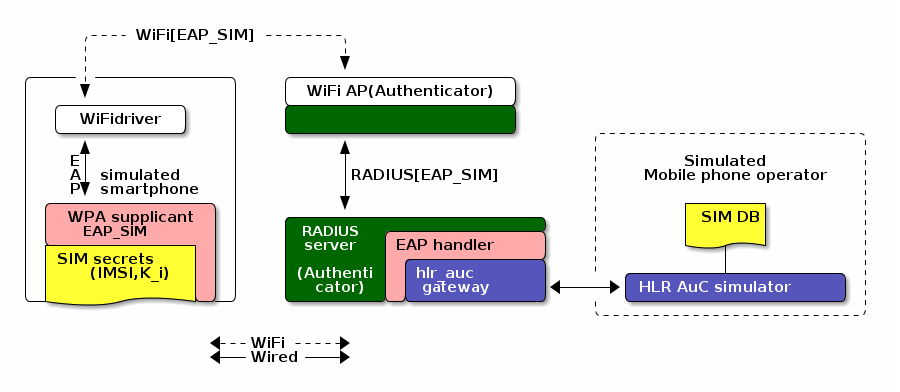
\includegraphics[width=.9\linewidth]{demoinfra.png}
\caption{\label{eap-sim-testbed}EAP-SIM authentication test bed in simulation environment}
\end{figure}





Used physical devices are AP and laptop.
AP used is running OpenWRT firmware.

Laptop computer's software has WPA-supplicant for Wi-Fi access,
hostapd for wired connected RADIUS server and hlr\_auc\_gw for MNO's
HLR. Laptop's role is also physically split-brain: It asks  from
itself for AA. Logically the model can be better described in
figure\ref{eap-sim-testbed}.


Jouni Malinen's software package \emph{wpa} can be thought as an reference
implementation providing all necessary components: WPA-supplicant, Wireless
Access point (AP), HLR-gateway (for GSM networks) and EAP-endpoint with
or without RADIUS-server. HSS replaces HLR in 3G/UMTS networks.

For more realistic test, OpenWRT AP is used instead of \emph{wpa's} hostapd
and hostapd has provided only RADIUS server.
OpenWRT AP works as a RADIUS client connecting to RADIUS server. 
It will not try to open EAP-messages or need
to know about them, it just encapsulates them into RADIUS packet.

\section{Detailed description of test runs}
\label{sec-5-2}



Test run with hostapd and simulated HLR\_auc\_gw [draw picture], did
not go first as planned. First there was no indication of SIM method
present in captures, only indication of security was open access.
After some modifications, runs got to the authentication phase.
Naturally, challenge-responses did not work 
because simulated SIM and it's secrets were known. 
Examples in appendix \ref{app:nosim}   



Test runs were made with diverse clients.
\begin{itemize}
\item Nokia phone with Symbian 60 Series OS (2006) with keyboard
(wings model) had no SIM card. Despite that it took part in making
primary traffic.
\item Nokia e90 Symbian xx with registered SIM had better results. Traced
sim2 sim3 and in folder \verb~gitdocs/di/testit/~ files \verb~eap3.pcapng~,
\verb~e90.sim.auth.pcapng~ and \verb~eap-1.pcapng~
\item WPA-supplicant running on laptop had simulated SIM-card access
with SIM/USIM protocols, respective EAP-SIM and EAP-AKA.  
Information from software claimed that "Hostapd
will send SIM/AKA authentication queries over a UNIX domain socket
to an external program, e.g., \verb~hlr_auc_gw~." Appendix \ref{app:hlraucgw}
shows that traffic.
\end{itemize}
\begin{itemize}
\item Shell program\ref{app:fulleap} starts needed programs. It also records used configurations,
logs, and traffic captures for later analysis.
\end{itemize}

\section{Disconnecting the local controller and offline changes}
\label{sec-5-3}
[Limiting time and forced logout, for how long access provided to
management operations, or use fast-auth on following accesses]

After phone has been successfully connected to the management network,
all changes coming from 
phone are automatically applied. There should be a way to close
session after changes has been applied. Originally it was thought,
that session would stay open only for limited time, after phone would
be forced to logout or thrown away from management network and 
that idea should be kept in mind when final implementation is made.



Terminating session is not included in the original RADIUS protocol.
The root cause is, that 
messages originating from the RADIUS server are not
defined in the protocol and so AP as RADIUS client cannot receive
RADIUS server initiated disconnection messages. Additional extensions
such as Disconnect and Change-of-Authorization (CoA) packets, also
known as RADIUS Dynamic Authorization or RADIUS Disconnection
Message(DM),  have later been brought in\cite{rfc5176} to protocol by
diverse vendors, but they may not all be implemented on every device. 
Disconnect-Request is sent to UDP port 3799, so authenticator should
listen also that in addition of RADIUS UDP port 1812.






Time limited access can perhaps made with session-timeout parameter
in ACCESS-ACCEPT packet. (or ACCESS-CHALLENGE). Type field = "29":
This parameter tells the authenticator how many second the supplicant
can maximal have service. More specifically said "what action
authenticator should do after termination becomes" and it has values
of either 0 (default) or 1 (radius request), which would mean that
authenticator may send new ACCESS-REQUEST to RADIUS server.  [check
Delivery of RADIUS attributes section]

But that would eliminate direct auth-only RADIUS cases [ \emph{were there}
\emph{any? I don't remember what I meant by this. Maybe that we needed only}
/to have authentication for access which in turn enables modifications./]
Is it then that with value 0, authenticator does not send
ACCESS-REQUEST to RADIUS server, but client still can automatically send it without 
user's acceptance?
\begin{itemize}
\item forced logout, like in captive portals, where RADIUS is not used.
\item no straightforward solution exists within RADIUS
\item AP is programmable with luci, which is used in configuring routers. It also could run some existing WWW-access
portal [-> reference to \hyperref[text:nointernet]{No Internet connectivity} link is
\end{itemize}

Offline changes includes cases where smartphone is not at home or when
there is no internet connection available.





If connection to Internet is down, full SIM authentication will not
work, because it needs co-operation from Internet, namely from MNO.
Simple solution would be sending one-time password to predefined
phone via an SMS, but what entity would then check that?
Authenticating server, which has no internet connection should 
have way to check that one-time password received via SMS is correct.

Solution for this could be co-existing WWW-based authentication, that
is web-page where credentials could be entered.
Software would run in AP. Existing solutions for this are for example
Chillisoft or NoCatAuth. That means open access to the
portal site must be provided.

[Full authentication vs. Fast re-authentication]

[fast-reauth is one parameter on wpa-supplicant configuration: enable/disable]



Full authentication uses IMSI which is the identity of phone's SIM.
Fast re-authentication would use temporal identity TMSI, which 
could change each time request had been sent. Values
are cached on authenticator and round-trip and handling at HLR is
eliminated. 
IMSI is 14 or 15 digit long number and presented as a composition
of strings belonging to MCC(2 digits), MNC(2-3) and MSIN(10),
As for TMSI, it is composed of pseudonym and realm part.
TMSI is used instead of IMSI to protect subscriber from being
identified and also make life more difficult to radio interface
eavesdroppers\cite{imsi-tmsi}.

Fast reauth is usually used on
local roaming[\cite{xxx}].
Automatic login with fast-authentication means, that no HLR AuC
is used. Instead, same K\_aut and K\_encr keys  that were used in full-auth are used  as Master Key to generate new Master Session key.\cite[30]{rfc4186}


\section{Network traces (EAP, SIM, AUTH traffic analysis)}
\label{sec-5-4}
Wireless capture between WPA-supplicant and AP was made on
WPA-supplicant's end-point, before it left wireless card. Capture was
not made in monitoring mode, so not all 802.11 details in
data packets were captured.  Because the focus was not in the
radio channel but instead in the EAP messaging, that was not problem.
\cite{wireshark-capture}

[Captured wireshark sessions give insight here. Analyze them.
Packet capture of successful SIM-authentication with corresponding
parts of logs at WPA-supplicant, RADIUS server and packet captures 
802.1X, RADIUS and HLR. Maybe also remote syslog from access point.]

\begin{itemize}
\item flow of messages
\item timing
\item size
\item attributes
\end{itemize}

Even, when authentication would no complete fully, authenticator
receives identification claim from mobile which of course can 
be false (see sequence, and explain why).

\begin{itemize}
\item 1st id claim comes already on second EAP message, from
wpa-supplicant to AP, working set in simulated environment.
\item date: 150123-155714
\item source: testit/demot/ap-s150123-155714/
\end{itemize}
\begin{verbatim}
Frame 129: 15:57:17.983047
    Type: 802.1X Authentication (0x888e)
    Version: 802.1X-2004 (2)
    Type: EAP Packet (0)
    Length: 5
    Extensible Authentication Protocol
        Code: Request (1)
        Id: 50
        Length: 5
        Type: Identity (1)
        Identity: 
Frame 130: 15:57:17.983223
    Type: 802.1X Authentication (0x888e)
    Version: 802.1X-2001 (1)
    Type: EAP Packet (0)
    Length: 21
    Extensible Authentication Protocol
        Code: Response (2)
        Id: 50
        Length: 21
        Type: Identity (1)
        Identity: 1232010000000000
\end{verbatim}

Note: AP uses version 802.1X-2004 while WPA-supplicant responses with
version 802.1X-2001. There should be no differences.

Identity is filled in wpa-supplicant both
in identity and cred section.

TO DO: Check other examples, where  they are not the same!

Last: not shown here, but Identity is not numerical but string.
[Reminds me of encoding IP addresses as strings in DNS request instead of bytes.]

\begin{verbatim}
# EAP-SIM with a GSM SIM or USIM
beacon_int=10
#
network={
        ssid="simtest"
        key_mgmt=WPA-EAP
        eap=SIM
#       pin="1234"
#       pcsc=""
  identity="1232010000000000"
  # leading "1" means use EAP-SIM. Other values "2" EAP-AKA and "6" EAP-AKA'
  # identity="2232010000000000"
  # and milenage parameters
  password="90dca4eda45b53cf0f12d7c9c3bc6a89:cb9cccc4b9258e6dca4760379fb82581"
}

cred={
        imsi="1232010000000000"
        milenage="90dca4eda45b53cf0f12d7c9c3bc6a89:cb9cccc4b9258e6dca4760379fb82581"
}
\end{verbatim}

This identity is wrapped into RADIUS packet and is sent to RADIUS
server:
\begin{verbatim}
Frame3: 15:57:17.988616
Radius Protocol
    Code: Access-Request (1)
    Packet identifier: 0xa2 (162)
    Length: 193
    Authenticator: 055ff370b9e793c1e39d375aade8033c
    Attribute Value Pairs
        AVP: l=18 t=User-Name(1): 1232010000000000
        AVP: l=7 t=NAS-Identifier(32): musta
        AVP: l=27 t=Called-Station-Id(30): 66-66-B3-8A-68-B3:simtest
        AVP: l=6 t=NAS-Port-Type(61): Wireless-802.11(19)
        AVP: l=6 t=NAS-Port(5): 1
        AVP: l=19 t=Calling-Station-Id(31): 5C-51-4F-E7-FA-F4
        AVP: l=24 t=Connect-Info(77): CONNECT 54Mbps 802.11g
        AVP: l=19 t=Acct-Session-Id(44): 5491885C-00000037
        AVP: l=6 t=Framed-MTU(12): 1400
        AVP: l=23 t=EAP-Message(79) Last Segment[1]
            EAP fragment
            Extensible Authentication Protocol
                Code: Response (2)
                Id: 50
                Length: 21
                Type: Identity (1)
                Identity: 1232010000000000
        AVP: l=18 t=Message-Authenticator(80): 04ea7e507d72bdb1acf515ef19ac9527
\end{verbatim}
Interesting part is the EAP fragment, having
Identity="1232010000000000", but
also RADIUS message itself, where User-Name field has been set also 
to "1232010000000000". Maybe this has something to do with identity
values above, or then AP just has followed conventions on converting
EAP into RADIUS message. The last RADIUS Attribute Value Pair (AVP) is 
Message-Authenticator, which presents limited safe against message 
corruption. Limited, because it uses MD5-hashing which is not safe
against malicious use anymore.





ks. /home/itapuro/gitdocs/di/testit/demot/ap-s150123-155714


\chapter{Analysis, Results and Discussion}
\label{sec-6}


\section{Deployment difficulty}
\label{sec-6-1}

To deploy the system, modifications must be done to AP and client.
Additionally, contract must be made to service
provider producing AuthN while AuthZ is already taken care of with cloud service contract.
For AP, modifications are minimal. Needed settings are
WPA mode to enterprise, IP-address of RADIUS server providing 
AA, and corresponding shared secret.
For client, Wi-Fi profile must be added: used SSID for management,
protection mode 802.1X (or WPA-Enterprise), AuthN method EAP-SIM.
Smartphone modifications can exist together with other
profiles, different SSID makes that separation possible.

Local tests, with software back ends need < 20ms for EAP-RADIUS message
exchange. 
Add there scanning of Wi-Fi network, SIM card's computing
time [take reference on network authentication part on earlier
tests. Timeout was 3 seconds for that part.]
Some figures for authentication times can give comparison to eduroam
or LANGATONWPA WPA network through couple RADIUS proxies in between home
organization's RADIUS service.

\section{Costs for end-user}
\label{sec-6-2}
\begin{itemize}
\item Cost per authentication from MNO. Mobiilivarmenne
currently is free for clients (personal use), but how about costs
for  service providers?
\item Hardware. Phones included.
\item Can EAP-SIM be used for other areas to divide costs?
\end{itemize}

Because only MNO and SIM-card manufacturer know 
what are SIM's K\_i and used A3/A8 algorithm
for GSM/3GPP/LTE authentication,
EAP-SIM always needs MNO for first authentication.


Idea: Divide secret for part that implements auth for own operator and
for part, that is free to use. What is the anatomy of SIM card?  How
about MULTI-SIM cards? (Multi-SIM service = 2 cards with same IMEI,
where Operator chains calls.)  For normal mobile phones, Dual-SIM
allows change of ID for example between work and private. Also:
\begin{quote}
"saving money by combining two different plans or  network carriers." 
\end{quote}

Same functionality can be achieved in DualSIM by prefix code before
private calls in modern phones while early versions required 
phone booting.

Multi-SIM cards have not been tested in this thesis, but one supposes
that they would show themselves as two separate identities as 
phone itself is not used in AA. It only reveals  MAC-address of its
radio interface, but that is not used in EAP-SIM AuthN unlike in MAC-based web-access portals.


\section{Platform specific issues: eg memory requirements, hardware requirements, computation requirements}
\label{sec-6-3}

For clients: 
\begin{itemize}
\item no need for PKI (in WPA, how wpa-supplicant checks RADIUS server's
authenticity?). Compare algorithms used in EAP-SIM A3/A8 (aka
COMP128 v1,2,3) to those of
TLS computation to RSA, SHA, cite from publication.
Which version was used in demo? V1 has been discontinued since 2002.

\item Considering WPA-supplicant + Hardware access to SIM,
at least few years ago there were not support for Android + SIM
auth \cite{android-sim}, although EAP-SIM (and -AKA) methods do
work at least on Android 4.x:
\end{itemize}
\url{http://www.ida.gov.sg/Infocomm-Landscape/Infrastructure/Wireless/Wireless-at-SG/For-Consumer/SIM-based-Connection-Guide}


From t.j.c: (jolla), what is needed to bring EAP-SIM support
to smartphone Jolla:
"Symbian also support EAP-SIM (at least S60r5, tested successfully on 5800 XpressMusic).

\begin{itemize}
\item add pcsc-lite package (needed to access SIM card)
\item compile wpa\_supplicant package with EAP-SIM support (needs pcsc-lite according to doc)
\item\relax [update connman to handle EAP connections]
(Triton (Jan 6 '14))"
\end{itemize}

This comment is in line, what was done in testing, without pcsc-lite
because SIM card was not used but a file.

Besides Switzerland (Swisscom), in South Korea every mobile operator
use EAP-SIM for their authenticated Wi-Fi connection.
(source t.j.c peremen (Jan 27 '14)"



For platforms (OpenWRT):
\begin{itemize}
\item OpenWRT is environment for embedded system.
When software is not fully optimized, memory is one of the limits which come first.
Base  wpa software is less than 128k, but 
that does not include RADIUS server part nor EAP-SIM.
\end{itemize}

Software limitations: 
\begin{itemize}
\item Freeradius2 is not included yet in OpenWRT.
\end{itemize}
It would also be based heavily on current Perl environment which
itself may be a space hog. 
Currently, as of 1.7.2014, there is no support for EAP-AKA on
freeradius2 even when there was on version 1.1.4.
(\url{https://github.com/FreeRADIUS/freeradius-server/blob/master/src/modules/rlm_eap/libeap/comp128.c} )
Yet, Freeradius can be used as Authentication Center (AuC).
\begin{itemize}
\item Diameter (freeDiameter) can be compiled in OpenWRT. That is good,
\end{itemize}
because Diameter protocol has more support on 3GPP than RADIUS.
\begin{itemize}
\item If nothing else works, as a backup old-fashioned
\end{itemize}
WWW-authentication portal can be used for offline authentication.

It does not take much space to save admin IMSI which is 15 digits at
most. 
As $2^{50} = 1125899906842624$
then 50 bits is smallest amount of bits needed to encode 16 digit long
decimal in binary. So 15 digits can be encoded with
50 bits,  and it takes no more than seven bytes (not 15) to save that
information as can be seen in equation\ref{eq:encoding}.

In reality, such optimization only leads to misunderstandings, if
context gets lost. Other information is also needed, for example
time stamps and accounting logs so these calculations are not precise.

\begin{equation}
 \label{eq:encoding}
  \left \lceil \frac{50}8 \right \rceil \frac{bits}{bits/bytes} = \\
   \left \lceil 6.25 \right \rceil bytes = 7~{}bytes
\end{equation}

\section{Discussion}
\label{sec-6-4}

The environment is modern complex home network management.
Configuration management tools are 
external in the cloud. Trust between homenet and cloud is searched.
Smartphone lies in the intersection of both domains 
and possess properties to simplify binding of that trust.
SIM card of smartphone, used together with Wi-Fi access to homenet 
verifies change controls. For verification, there are few options presented.

Location of AuthN and AuthZ components may also vary.
Always in the beginning, AuthN lies outside homenet, but
later it can use local point. AuthZ may be located more freely.
RADIUS directs user into own virtual LAN segment (VLAN),
and there management of homenet devices is allowed.
That procedure activates the management port as of 802.1X standard
specifies.
Thesis thus uses old, yet simple method for problem risen in modern environment homenet.

Disconnection from normal (Wi-Fi) access network happens, before phone can get
into management network. It means, that all stateful network
connections using Wi-Fi will close at that point. Smartphones do not
have multiple wireless connections, but mobile data connections may 
stay up. Even then, the default routing in the smartphone may change.

In the theory chapter it was questioned whether proxying RADIUS server
can read and alter messages on their way or is the messaging secured
by encryption, integrity hashes and digital signatures.
Later it was learned, that message's integrity is protected but not encrypted.

EAP does by definition only AuthN part although successful
authentication often precedes ad hoc AuthZ if nothing is demanded.
EAP-SIM handles this part, but for AuthZ something else is needed
and so some methods has been presented to add right role to 
authenticated identity.
\section{Security considerations}
\label{sec-6-5}



There can be multiple ways to attack described methods of
homenet management delegation. Following divides them into
Confidentiality (privacy), Integrity (tampering), and
Authenticity, Accessibility is also discussed.


The purpose of message confidentiality in authentication phase is
to hide identity and possible delivered secrets from
eavesdroppers. EAP-SIM cannot be considered confidential during 
first message exchanges, but later identity can be hidden.
There are no mitigation for revealing the IMSI on the first message,
This can be compared with regular GSM network identity revealing: IMSI
catching is a concept of listening radio network for phones that are
powered on and register themselves to operator via GSM network.  

The
fault lies there, that GSM specification does not require network to
authenticate itself to the phone thus GSM allows man in the middle
attack device called IMSI-catcher to fake as being a base station.
When mobile phone tries to attach to fake base station, it reveals its
IMSI number. Further, because the base state is responsible for chosen
encryption, it can order phone to not encrypt traffic or to use only
weak encryption thus revealing all data, calls, and
texts\cite{imsi-heise}. Mitigation for IMSI-catching would be to
disable GSM (2G) usage altogether from phone if that is possible.




Integrity issues were handled in RADIUS section \ref{section:radius}.
Message digestion codes provide integrity for RADIUS-protocol.
If PEAP is used, it handles integrity through its usage of TLS\cite{peap}.

\section{Accessibility, DoS and Scalability}
\label{sec-6-6}
Is homenet immune against (distributed) denial of service (DoS)
attacks? Besides DoS, does the solution scale up from on homenet to
small and middle size companies?
To answer this we can remember that backends (cloud and operator) are
designed for thousands or even millions of concurrent users, so 
they hardly are limiting factor. Instead, local
authenticator might suffer from inefficiency, which
comes from processing loads\cite{2009-lin-simefficiency}.


Traditionally, RADIUS has used connection-less UDP protocol for its
light weightiness. UDP misses reliability, but retransmission in UDP is
tolerable, because user is ready to wait several seconds for
authentication to complete. Today, RADIUS can also run over TCP, which
has generally more aggressive retransmission
rate\cite[2.2.1]{rfc5080}. On the other hand, use of an alternate
RADIUS server serves better than waiting for TCPs reliable delivery.



\section{RADIUS weaknesses and strengths in limited use cases}
\label{sec-6-7}


RADIUS protocol itself is old and not very secure as of current
standards(2015), because messages are not encrypted and they are
transported on datagrams (UDP). Alternative RADSEC protocol uses TLS, and 
is compatible backwards to RADIUS protocol, so it can be used
as secure RADIUS proxy\cite{uninett-radproxy}.

RADIUS uses MD5 hashing and shared secrets. Because of weaknesses of
MD5-hashing (MD5Attack\cite{rfc5176}), the transport needs additional protection like
tunneling or IPsec. TLS can be used encryption and
signatures, although there are some integrity checks built into the
RADIUS-protocol itself.
RADIUS messages are protectected from basic 
message injection without previous knowledge by those integrity checks,
and they use session secrets, hashes and XOR.


In scenario \ref{scenario-iii}, there is proxying RADIUS between authenticator
and MNO.  When MNO notifies Authenticator
that an user has been authenticated, then authenticator (AP, functioning
as a RADIUS-client) hooks that message and usually just grants smart
phone access to network. After giving access rights, other
provisioning parameters can be sent with RADIUS messages, for example
Session Time-out,
current admin user list, state of OTP list, or VLAN id.

Earlier in RADIUS analysis, prevention of replied messages was
mentioned. Reusing same secret in different security context is also
considered bad.  Mixing secrets between usage
domains weakens them.  In GSM networks, IMSI identifies subscriber on
first contact, later TMSI is used for call and SMS.  In EAP-SIM those
values are also used. IMSI naturally is same, but TMSI should be
different for call and EAP.  Haverinen\cite{hav-doc} explains how
special RAND numbers can be used to differentiate use of 3GPP and LAN
contexts.

Re-authentication and termination can bring unexpected results.
If SSID changing, which was introduced in mitigation section(\ref{tag:hidessid}) was in use, fast re-authentication
should be forbidden\cite[p.11]{rfc5448}.
Even, when sessions can be terminated, the client side have 
option to login automatically, transparent and without users control.
Automatic re-authentication after disconnection  must be considered
here as harmful as well as automatic login. For example,
Swiss mobile operator Swisscom provided two networks for its customer:
"Mobile" and "Mobile Eapsim". The latter network did not ask customer
for connection and used smart phones SIM automatically. Unfortunately,
it also charged users for using Wi-Fi connections without their 
knowledge.\cite{swisscom}





If one can read and write data through SIM card's API,
he could try to get information (SRES, K\_c) by using the card as an
oracle[def]. Fortunately SRES and K\_c are never sent in clear but
inside AT\_MAC. Additionally SIM card can be programmed to answer only
limited amount of challenge request, for example 65535, which in
normal usage would be enough, but in brute-force challenges 
would soon fill up.


\section{Mitigation methods}
\label{sec-6-8}
To mitigate risks two methods are presented: Hiding of
wireless network and proximity. They are not perfect but can
limit attack vectors in time and place.

Recall that the management network is needed only then when changes
are challenged. Why then not just enable management radio network
then? Then there were less networks for users to choose from.
Enabling management network could be achieved by lUCI-interface, but
it also may need disruption of all Wi-Fi access and restart of AP,
which certainly would not be wanted.  

\label{tag:hidessid}
One could also think of hiding the network by disabling the
advertisement of management network SSID, which is called "network
cloaking".  Smartphone would then need to know exactly the SSID name
to try to connect. The SSID could also be renamed always, in essence
to implement one-time-only Network, but then the smartphone would
need to get that secret somewhere, perhaps via an SMS, but then again
that would defeat the purpose of easy access.

Does disabling or hiding the management network bring real security or
is it just security by obscurity?  Security by obscurity means here,
that hiding network would be the only security method.
Disabling or hiding  merely gives one security layer more so it is not
real security method.

When the usage here is to always renew SSID name then
hiding actually could add security. AP does not reveal any information
before the client has tried to connect to it, so at least 
the time window for attacks is minimized. Indeed hiding can have
privacy enhancing effects: Lindqvist\cite{hidden-wlan} uses hidden APs
to protect privacy of clients who actively probe for visited APs and
would otherwise reveal their visited places.


Regarding boundaries of homenet, the Wi-Fi coverage gives 
one natural limit, which is 50 meters indoors or 100 meters outdoors,
when no extenders (i.e. repeaters) are in use.
Proximity so brings a minimal extra layer for preventing attacks
just like network cloaking as attacker must be physically within those limits.

[ add source
\url{http://compnetworking.about.com/cs/wirelessproducts/f/wifirange.htm} ]

This can be considered as an added factor in multifactor
authentication or reputation, but it will not be enough, because
attackers will have more sensitive  radios available than normal users devices have.(source?)
Also, if SIM-profile were used through Bluetooth, there were also
range limits, but even shorter.

\chapter{[MISC to be added on right places]}
\label{sec-7}


\section{More attacks from literature, not categorized}
\label{sec-7-1}
\begin{itemize}
\item dictionary and brute force not valid in EAP-AKA (rfc4187)
\item key size 128 or 64? (paper on key size "only 64bit, not 192bit")
\item VLAN itself has attack vector and some methods exists, but also
mitigation for them.
\item rad authenticator, TLS, RADSEC etc
\item Easily physically accessible devices are vulnerable to physical attacks.
\end{itemize}
\section{Second option for multirealms is using EAP-SIM or relatives (PEAP)}
\label{sec-7-2}
with \uline{user configurable} User and Domain parameters (-> pseudonym
protection), but as default, identity is read from SIM application (from
card).


\chapter{Conclusion}
\label{sec-8}




Homenet's future needs in configuration management have been
described. As an example, change of authority and delegation of
control to third parties are needs that have been presented.  A method to approve
changes indirectly has been proposed. The approval follows from
successful authentication and authorization with EAP-SIM method by
mobile phone. 
[ Connection to research work done on TUT pervasive
department's IoT project on homenets has also been presented. :TBD]



Complexity of existing models in interworking was one motivator for
the work. Research work on subject did reveal some of the reasons 
for the complexity, that are difficult to overcome with simplistic 
methods without in the same time losing some of security.


As results, a real working EAP-SIM test bed with fake credentials and
fake mobile operator representing EAP-SIM authentication flow has been
shown.  A dual-role model, which binds smartphone to homenet and
grants right to make changes has been proposed.  Working with
management network is indirect way to approve changes.  [or: An
indirect way to approve changes is achieved by binding authorized
access to management network.]


There are some obvious weakness in proposed solution. Possible usage
must carefully check the safety limits even when RADIUS-protocol still
has strengths in security today.
Thesis only scratches bootstrapping problems and 
work on bootstrapping the homenet needs to be studied more
thoroughly. One could use tickets in Kerberized way as in GBA. 
Software implementation as app is needed to the smartphone.

HS2.0  is promising point, it could also lead to
offloading of voice calls through local AP and Wi-Fi instead of radio net for
phones. Wi-FI - 3GPP offloading is subject for another study.
With proposed technique, provisioning of users at homenets would
minimize, as users already own an identifiable object, smartphone. As
a positive side effect, two-factor AuthN strengthens existing security.
Studying few steps further from here would bring 3GPP roaming on Wi-Fi
networks and that would be the missing link in interworking between
two worlds.




\newpage
\bibliographystyle{IEEEtranS}   % already on org header 

\renewcommand{\bibname}{Bibliography}     % Otherwise bilingual babel uses Finnish ``Kirjallisutta''. Strange...
\bibliography{refs}    % already on org header

\addcontentsline{toc}{chapter}{\bibname}  % Include this in TOC

\markboth{\bibname}{\bibname} % Set page header

% not needed \printbibliography                  
% a) heading in English


% if needed, appendix
\appendix
\pagestyle{headings}
%
% a) Not-so-handy way, but at least it works
% 
\def\appA{APPENDIX A. Scripts, confs, and logs} % Define the name and numbering manually
\chapter*{\appA}                       % Create chapter heading
\setcounter{chapter}{1} % Start numbering from zero because command

\markboth{\appA}{\appA}                % Set page header
\addcontentsline{toc}{chapter}{\appA}  % Include this in TOC
% Note that \label does not work with unnumbered chapter

Appendices are purely optional.  All appendices must be referred to in
the body text

%\thispagestyle{empty}
\section{shell, logging options}
\label{sec-8-1}
\label{app:fulleap}
\lstset{columns=fullflexible}
# % \lstinputlisting[language=bash]
\lstinputlisting[language=bash]{./testit/apd-tty.clean}



\section{wpa-supplicant creds}
\label{sec-8-2}
[already in text]
If KEYS have been excluded from log files, there as placeholder stays
string "[REMOVED]".
\lstinputlisting[language=sh]{testit/wpa-simtest-owrt2.conf.clean}

\section{RADIUS server conf}
\label{sec-8-3}
\lstinputlisting[language=sh]{testit/hostapd-jmdemo.conf.clean}
\section{hlr auc}
\label{sec-8-4}
\label{app:hlraucgw}

\section{No sim}
\label{sec-8-5}
\label{app:nosim}

Here capture + analysis from nosim
% Emacs 24.4.1 (Org mode 8.2.10)
\end{document}